\section{Design, Evaluation, and Usage}
\label{sec:eval}

In this section, we focus on the choices that influenced our design
(Section~\ref{sec:design}), we evaluate these choices in an existing
Liquid Haskell benchmark of programs (Section~\ref{sec:eval-eval}),
and demonstrate the usage of our tool with a small example
(Section~\ref{sec:example}).

\subsection{Design Choices}
\label{sec:design}

\begin{figure*}
  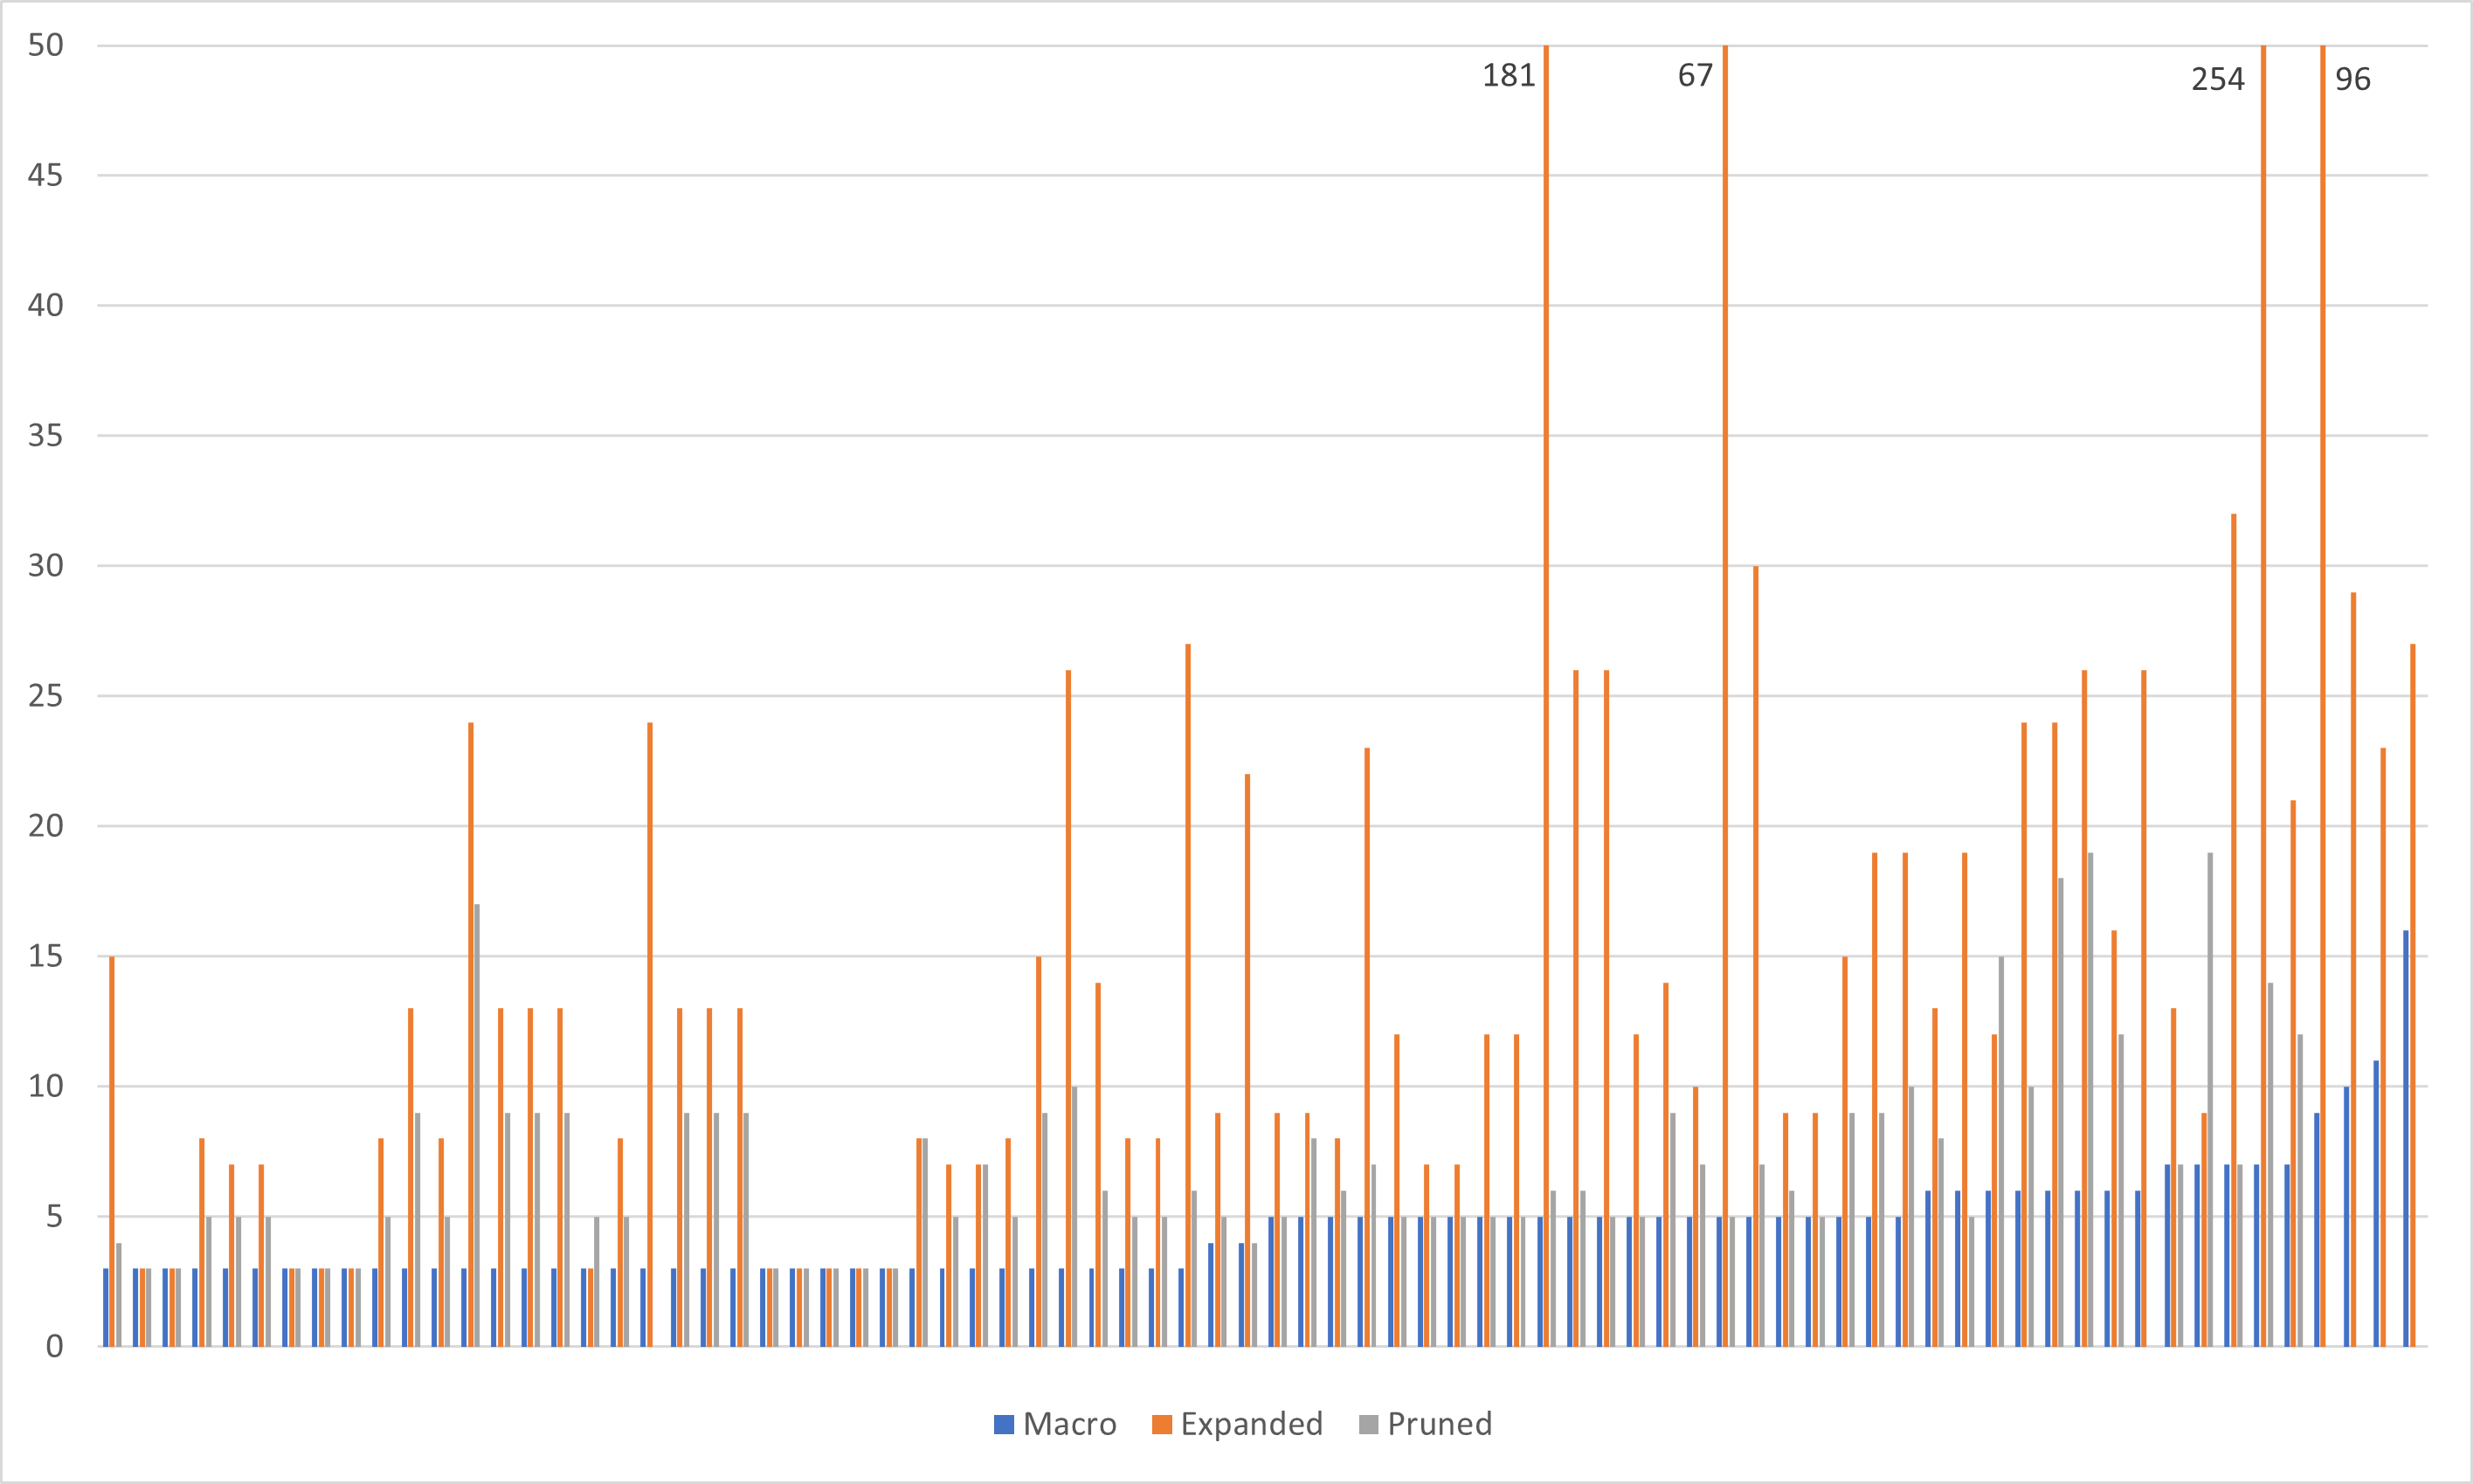
\includegraphics[width=\textwidth]{LiquidProofEval.png}
  \caption{LoC across benchmarks of Liquid Proof Macros (in \textcolor{blue}{blue}), the expanded splice (in \textcolor{orange}{orange}), and the minimal
    Liquid Haskell proof term (in \textcolor{gray}{gray})}
  \label{fig:loc-eval}
\end{figure*}

% % ? BEGIN OUTLINE

% The benefits we aim to provide with these proof macros are:
% - conciseness: the macros cater towards a specific subset of LH that is used
%   for extrinsic-style proofs, so the interface to this subset can be more
%   specific and restricted than generic programs
% - reduced redundancy: often, multiple logical branchings can be handled by the
%   same proof macro (due to the modularity the macros achieve in a similar
%   style to tactics), and proof macro branchings (such as destruct, induct,
%   condition) allow the handling proof macro to be written just once and then
%   used in all of the branches
% - modularity: in the same style as tactics, the auto proof macro is contextual
%   and so the same use of auto can be used to solve many different proof goals
%   by leveraging contextual information such as the lemmas, variables, and
%   sound recursions.

% To verify the applicability of these benefits, we selected an
% independently-curated collection of properties to be proved in an extrinsic
% style using Liquid Haskell: https://github.com/mustafahafidi/qc-to-lh. The
% original use of these properties was to demonstrate the usefulness of another
% approach to generating Liquid Haskell proofs that has some similarities to our
% approach.

% TODO: describe similarities and differences The properties are relatively
% basic properties about the natural numbers, lists of natural numbers or pairs
% of natural numbers, and trees of natural numbers.

% % ? END OUTLINE

When designing Liquid Proof Macros, we wanted users to benefit along the following three axis:

\paragraph{Conciseness.}
%
Extrinsic proofs are mostly written in a particular subset of Haskell,
the \LangB. Using metaprogramming to generate terms in this subset we
would expect proofs to be shorter than when written out explicitly.
%
%\paragraph{Reduced redundancy.}
%
Moreover, as most proof assistant users are familiar with, often many
different branches of a proof can be handled by the same proof
strategy. Rather than requiring users to replicate the same proof term
in each branch, proof macros allow for writing such strategies once
and applying them across all branches.

\paragraph{Modularity.}
%
Even though many proofs can be encapsulated by the same proof strategy
(e.g. simple induction), vanilla Liquid Haskell requires that strategy
to be written out in full verbosity in each instance (e.g.  pattern
matching on a list of a natural numbers, and then supplying the tail
or predecessor to the recursive call in the second cases
respectively). The proof macro system allows the user to modularly
encode proof strategies in such a way that the same sequence of proof
macros can be used to prove a wide variety of similar theorems that
use the same proof strategy.

\paragraph{Practicality}
%
The style of proof search used by our proof macro system is very
inefficient, verily because it includes all generatable neutral forms
(using a limited) context without using any sort of guided search. The
secondary pruning process, which is performed on a passing proto-proof
term after proof search is complete, aims to recover a minimal proof
term for the sake of readability and efficient re-checking.

\subsection{Evaluation}
\label{sec:eval-eval}

To evaluate our design, we turned to a prior benchmark suite of 80+
Liquid Haskell proofs~\cite{TacticThesis}, that consists of a
collection of boolean predicates over natural numbers, lists, and
binary trees, ranging from very simple facts to inductive properties
that require auxiliary lemmas. All proofs take advantage of both proof
macros, and {\em proof by logical evaluation}~\cite{VazouTCSNWJ18}, a
complementary technique for delegating some equational reasoning to
the SMT solver.

Using Liquid Proof Macros we were able to concisely prove ($<16$
LoC\footnote{Measured from the signature of the top-level function to the last
line of the macro sequence or proof term.} for all and $<10$ LoC for all but
two). Figure~\ref{fig:loc-eval} shows the lines of code across all such
benchmark using (1) Liquid Proof Macros (2) the expanded proof term (3) the
pruned minimal proof term. We found that in all cases proof macros where smaller
than the Liquid Haskell proof terms, with a (geometric) average of 57\%
reduction in LoC compared to the minimal pruned version. Moreover, to give an
estimate of the cost of proof search, the unpruned expanded splice generated by
Template Haskell was $2.88\times$ larger on average.


\begin{figure*}
  \centering

%  \begin{subfigure}[t][][t]{1\textwidth}
%   % \centering
%     \begin{minipage}[c]{0.5\textwidth}
%       \caption{The user writes the proof macros.}
%     \end{minipage}
%     \hfill
%     \begin{minipage}[c]{0.49\textwidth}
%       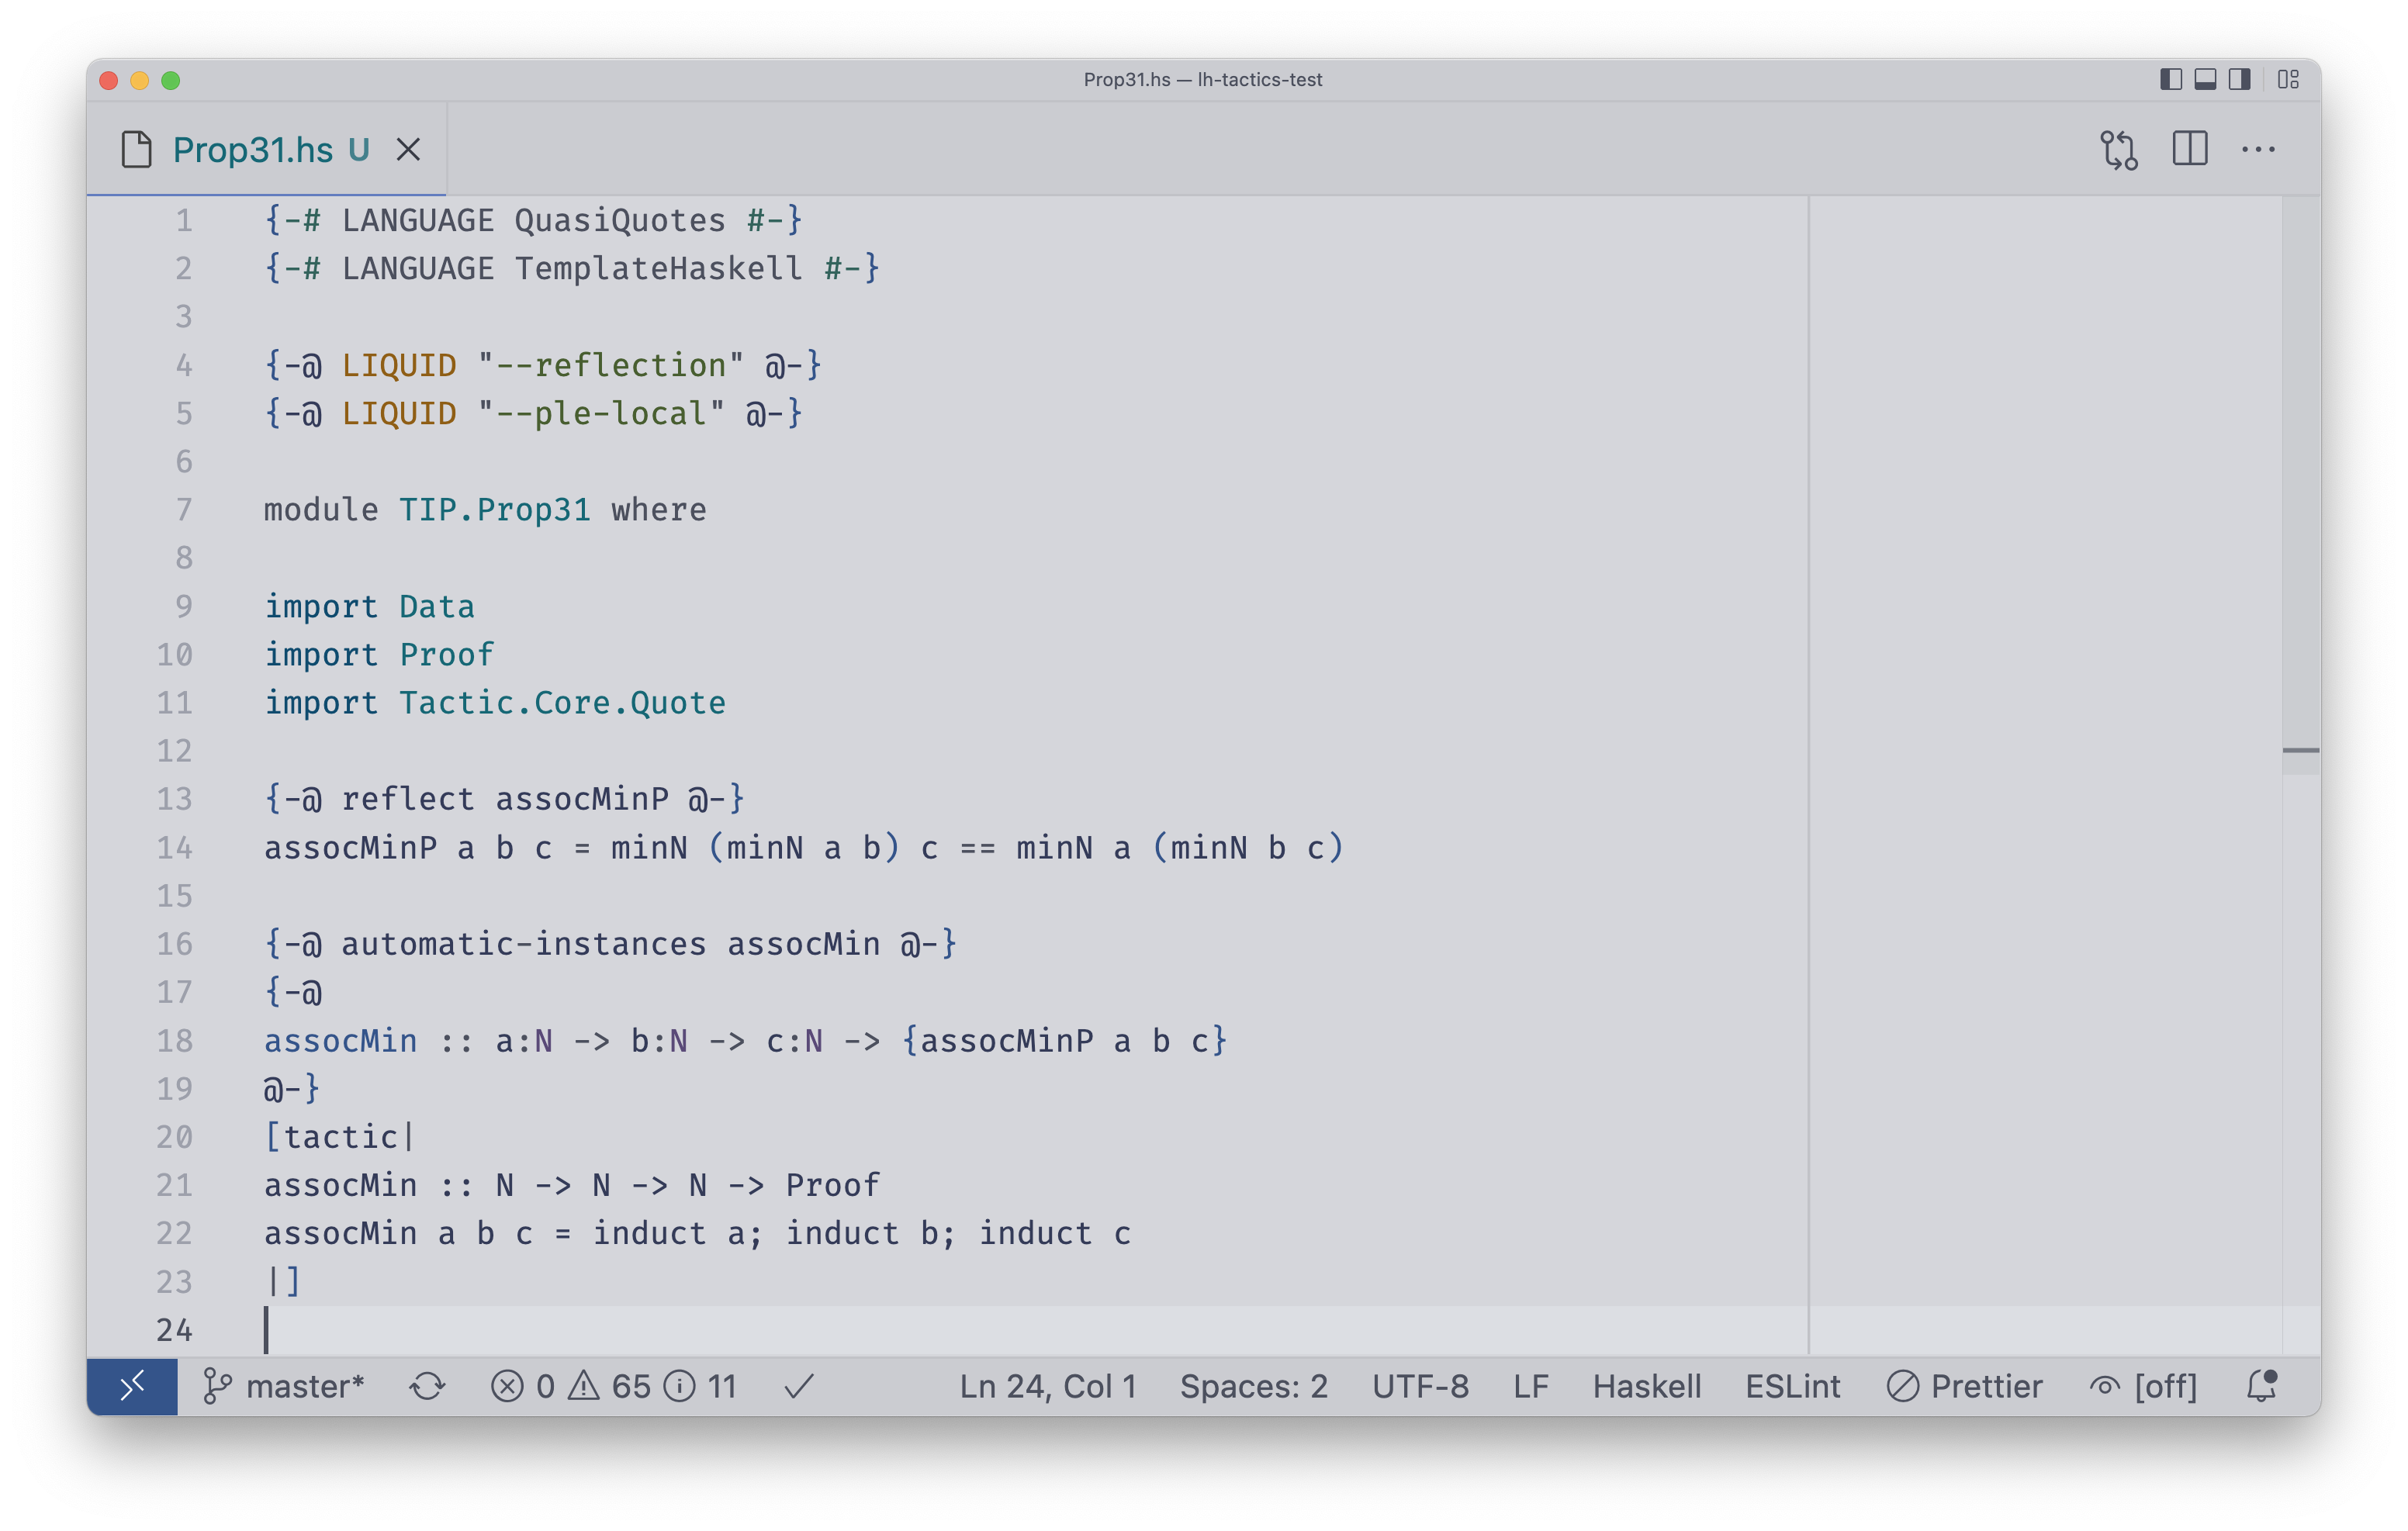
\includegraphics[width=\textwidth]{example-screenshots/macros.png}
%     \end{minipage}
%   \end{subfigure}
  \begin{subfigure}[t][][t]{1\textwidth}
    % \centering
    \begin{minipage}[c]{0.63\textwidth}
      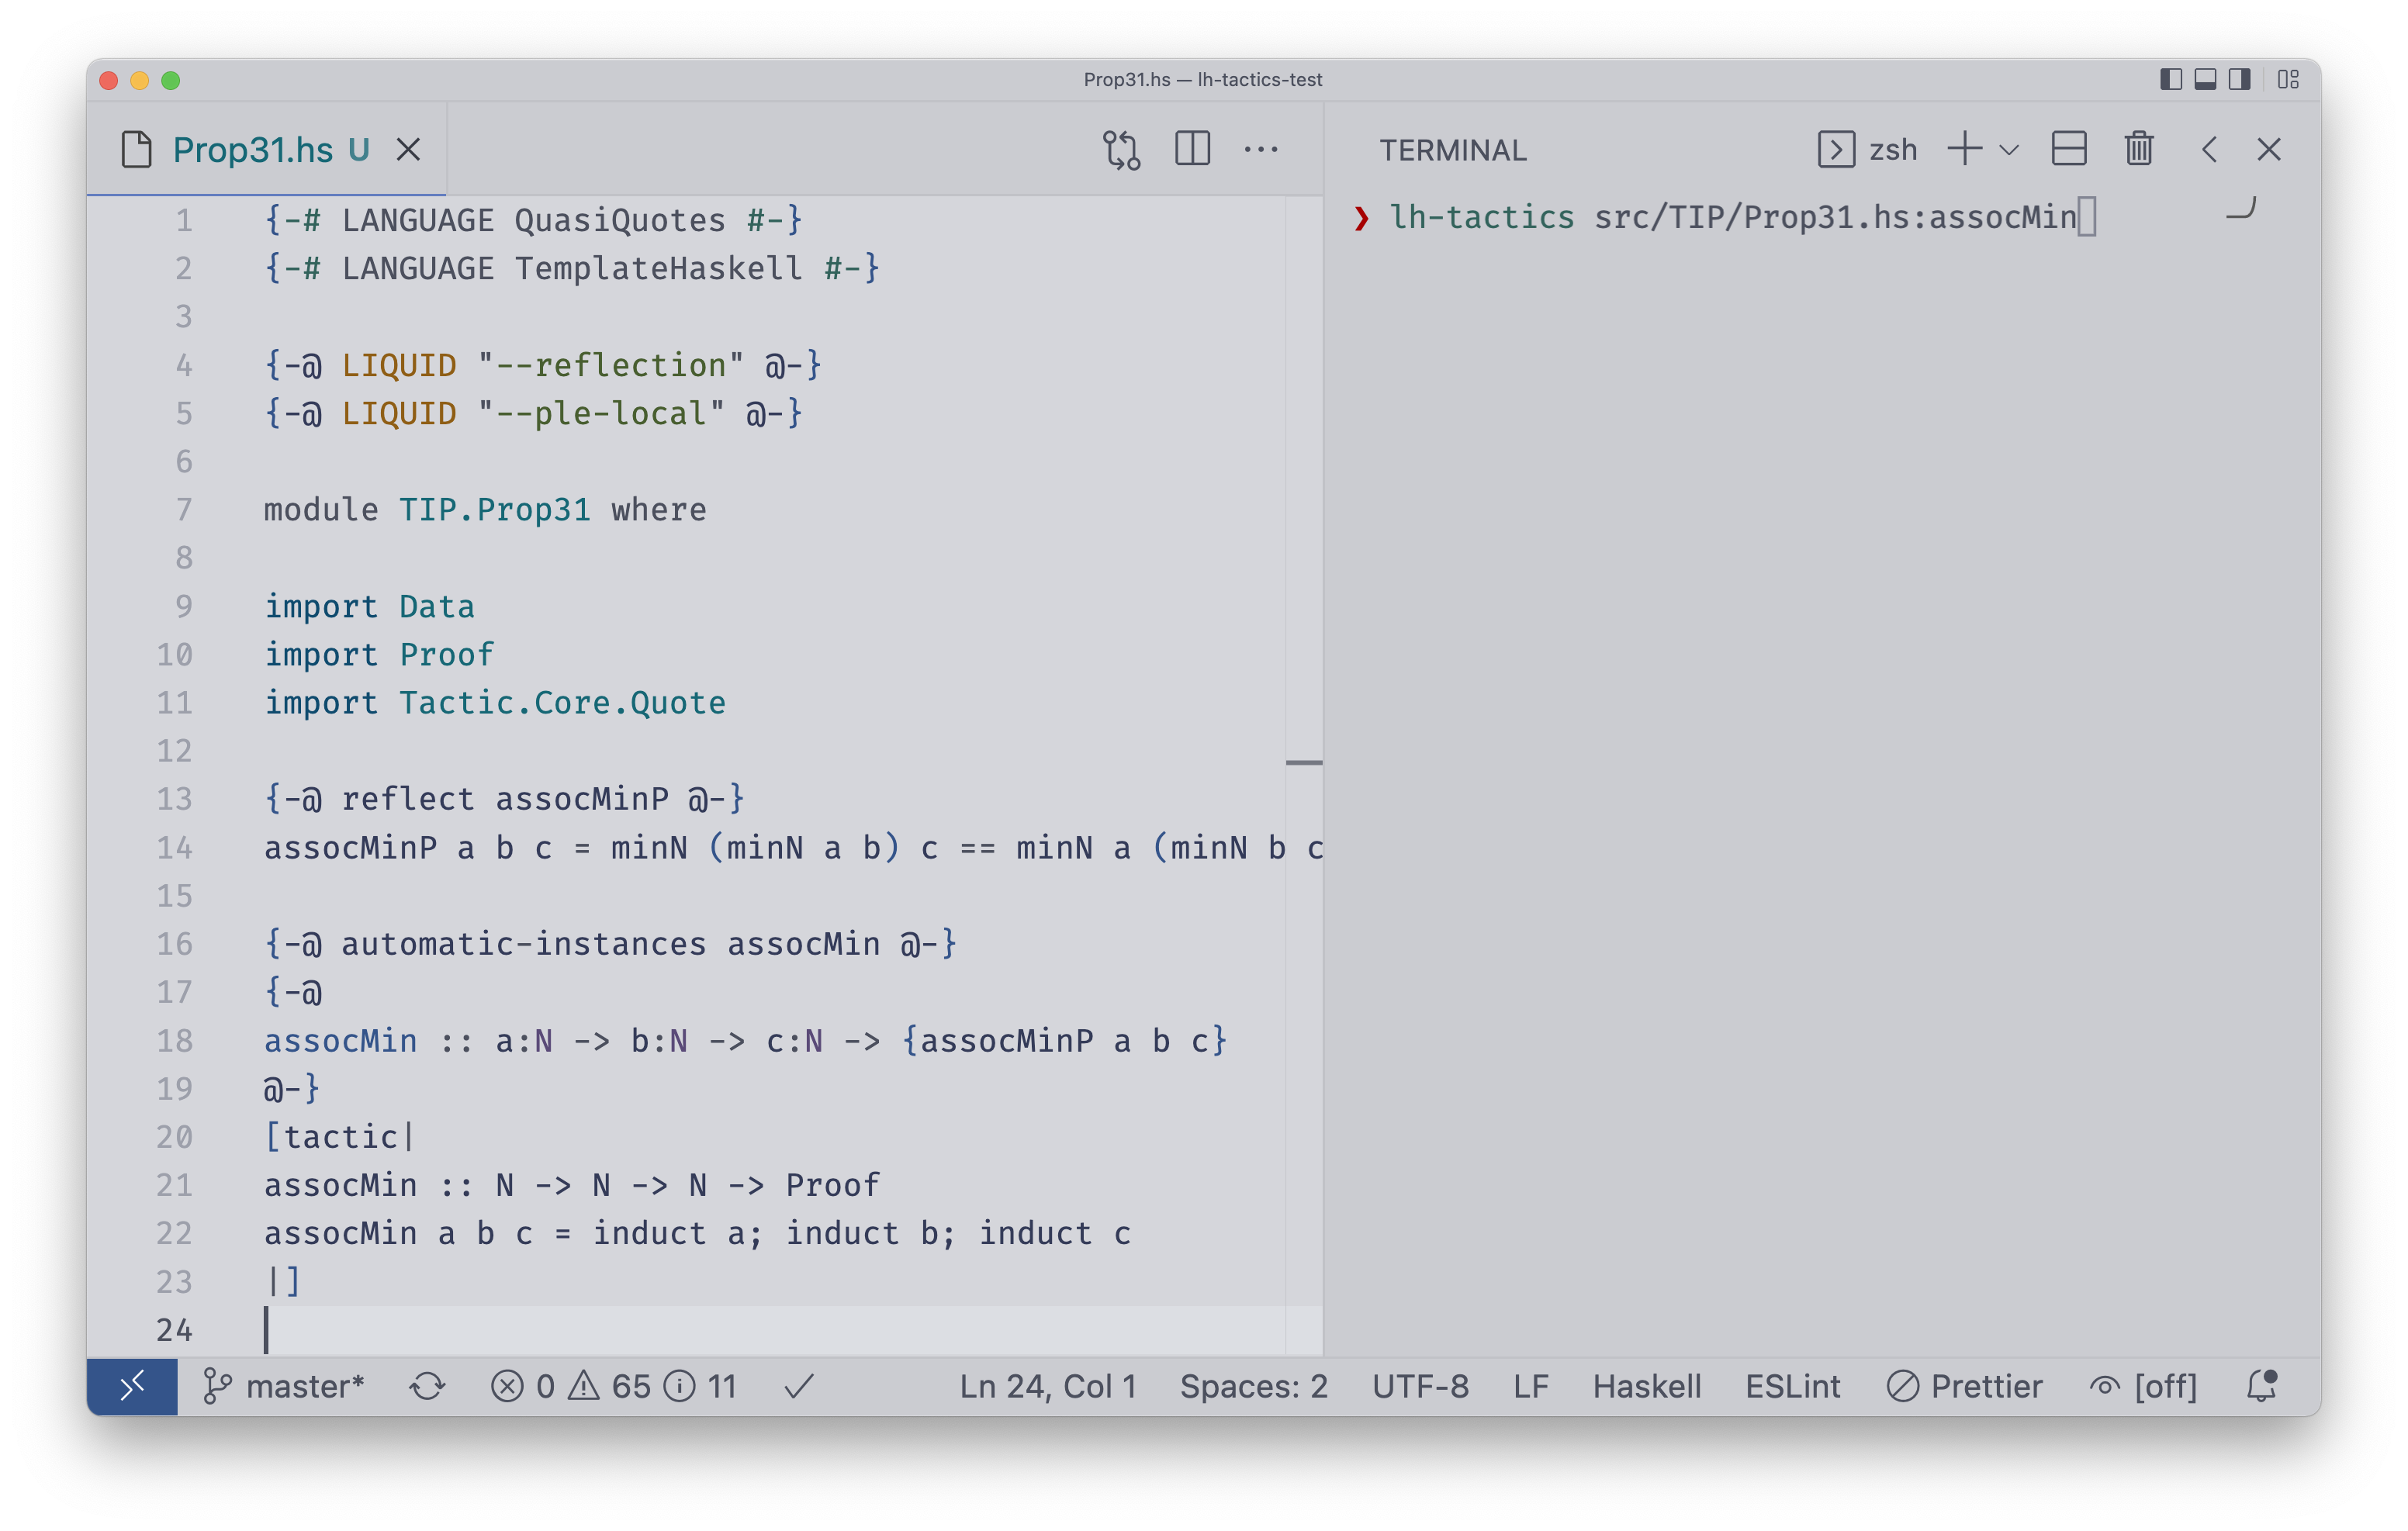
\includegraphics[width=\textwidth]{example-screenshots/run.png}
    \end{minipage} 
    \hfill
    \begin{minipage}[c]{0.3\textwidth}
      \caption{The user writes the proof macro and runs the
        \LC{lh-tactics} command line tool on the input file, which
        exists inside of a \textit{stack} project that is configured
        to use the LiquidHaskell as a plugin.}
    \end{minipage}
  \end{subfigure}
  \begin{subfigure}[t][][t]{1\textwidth}
    % \centering
    \begin{minipage}[c]{0.3\textwidth}
      \caption{The user waits for the \LC{lh-tactics} tool to complete. During
      this time, the tool will overwrite the input file on each pruning attempt.}
    \end{minipage}
    \hfill
    \begin{minipage}[c]{0.63\textwidth}
      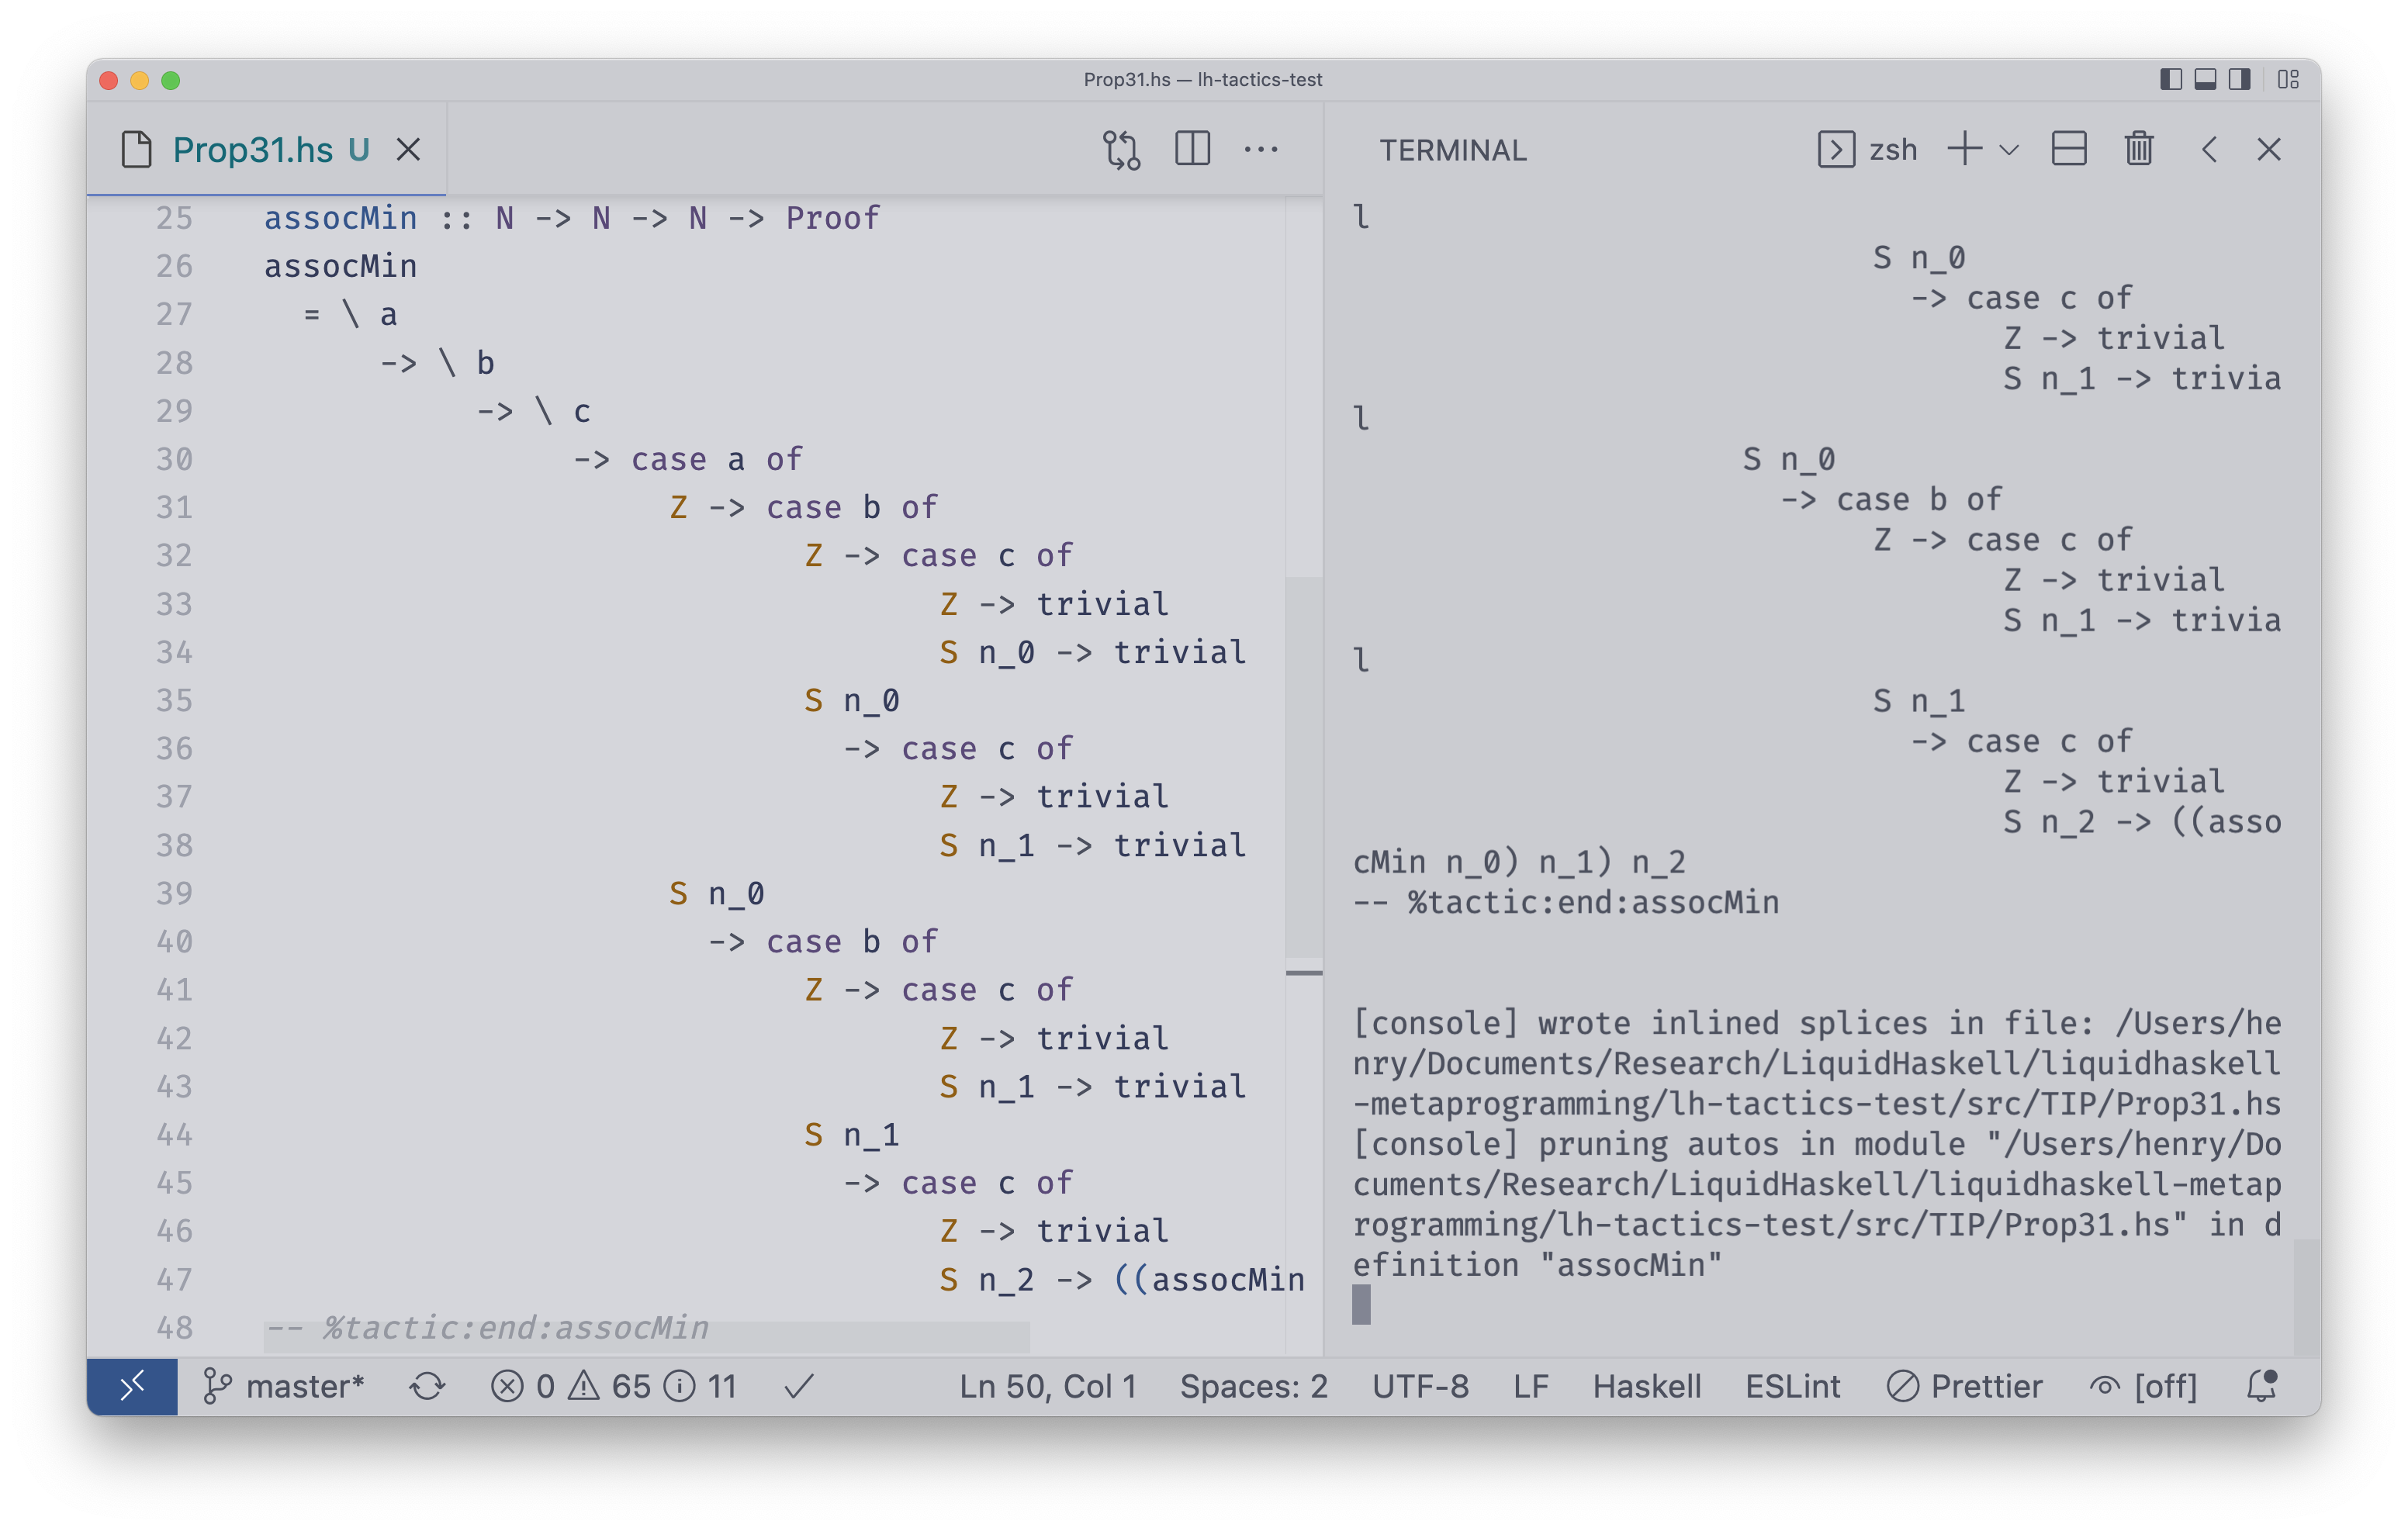
\includegraphics[width=\textwidth]{example-screenshots/pruning.png}
    \end{minipage}
  \end{subfigure}
  \begin{subfigure}[t][][t]{1\textwidth}
    % \centering
    \begin{minipage}[c]{0.63\textwidth}
      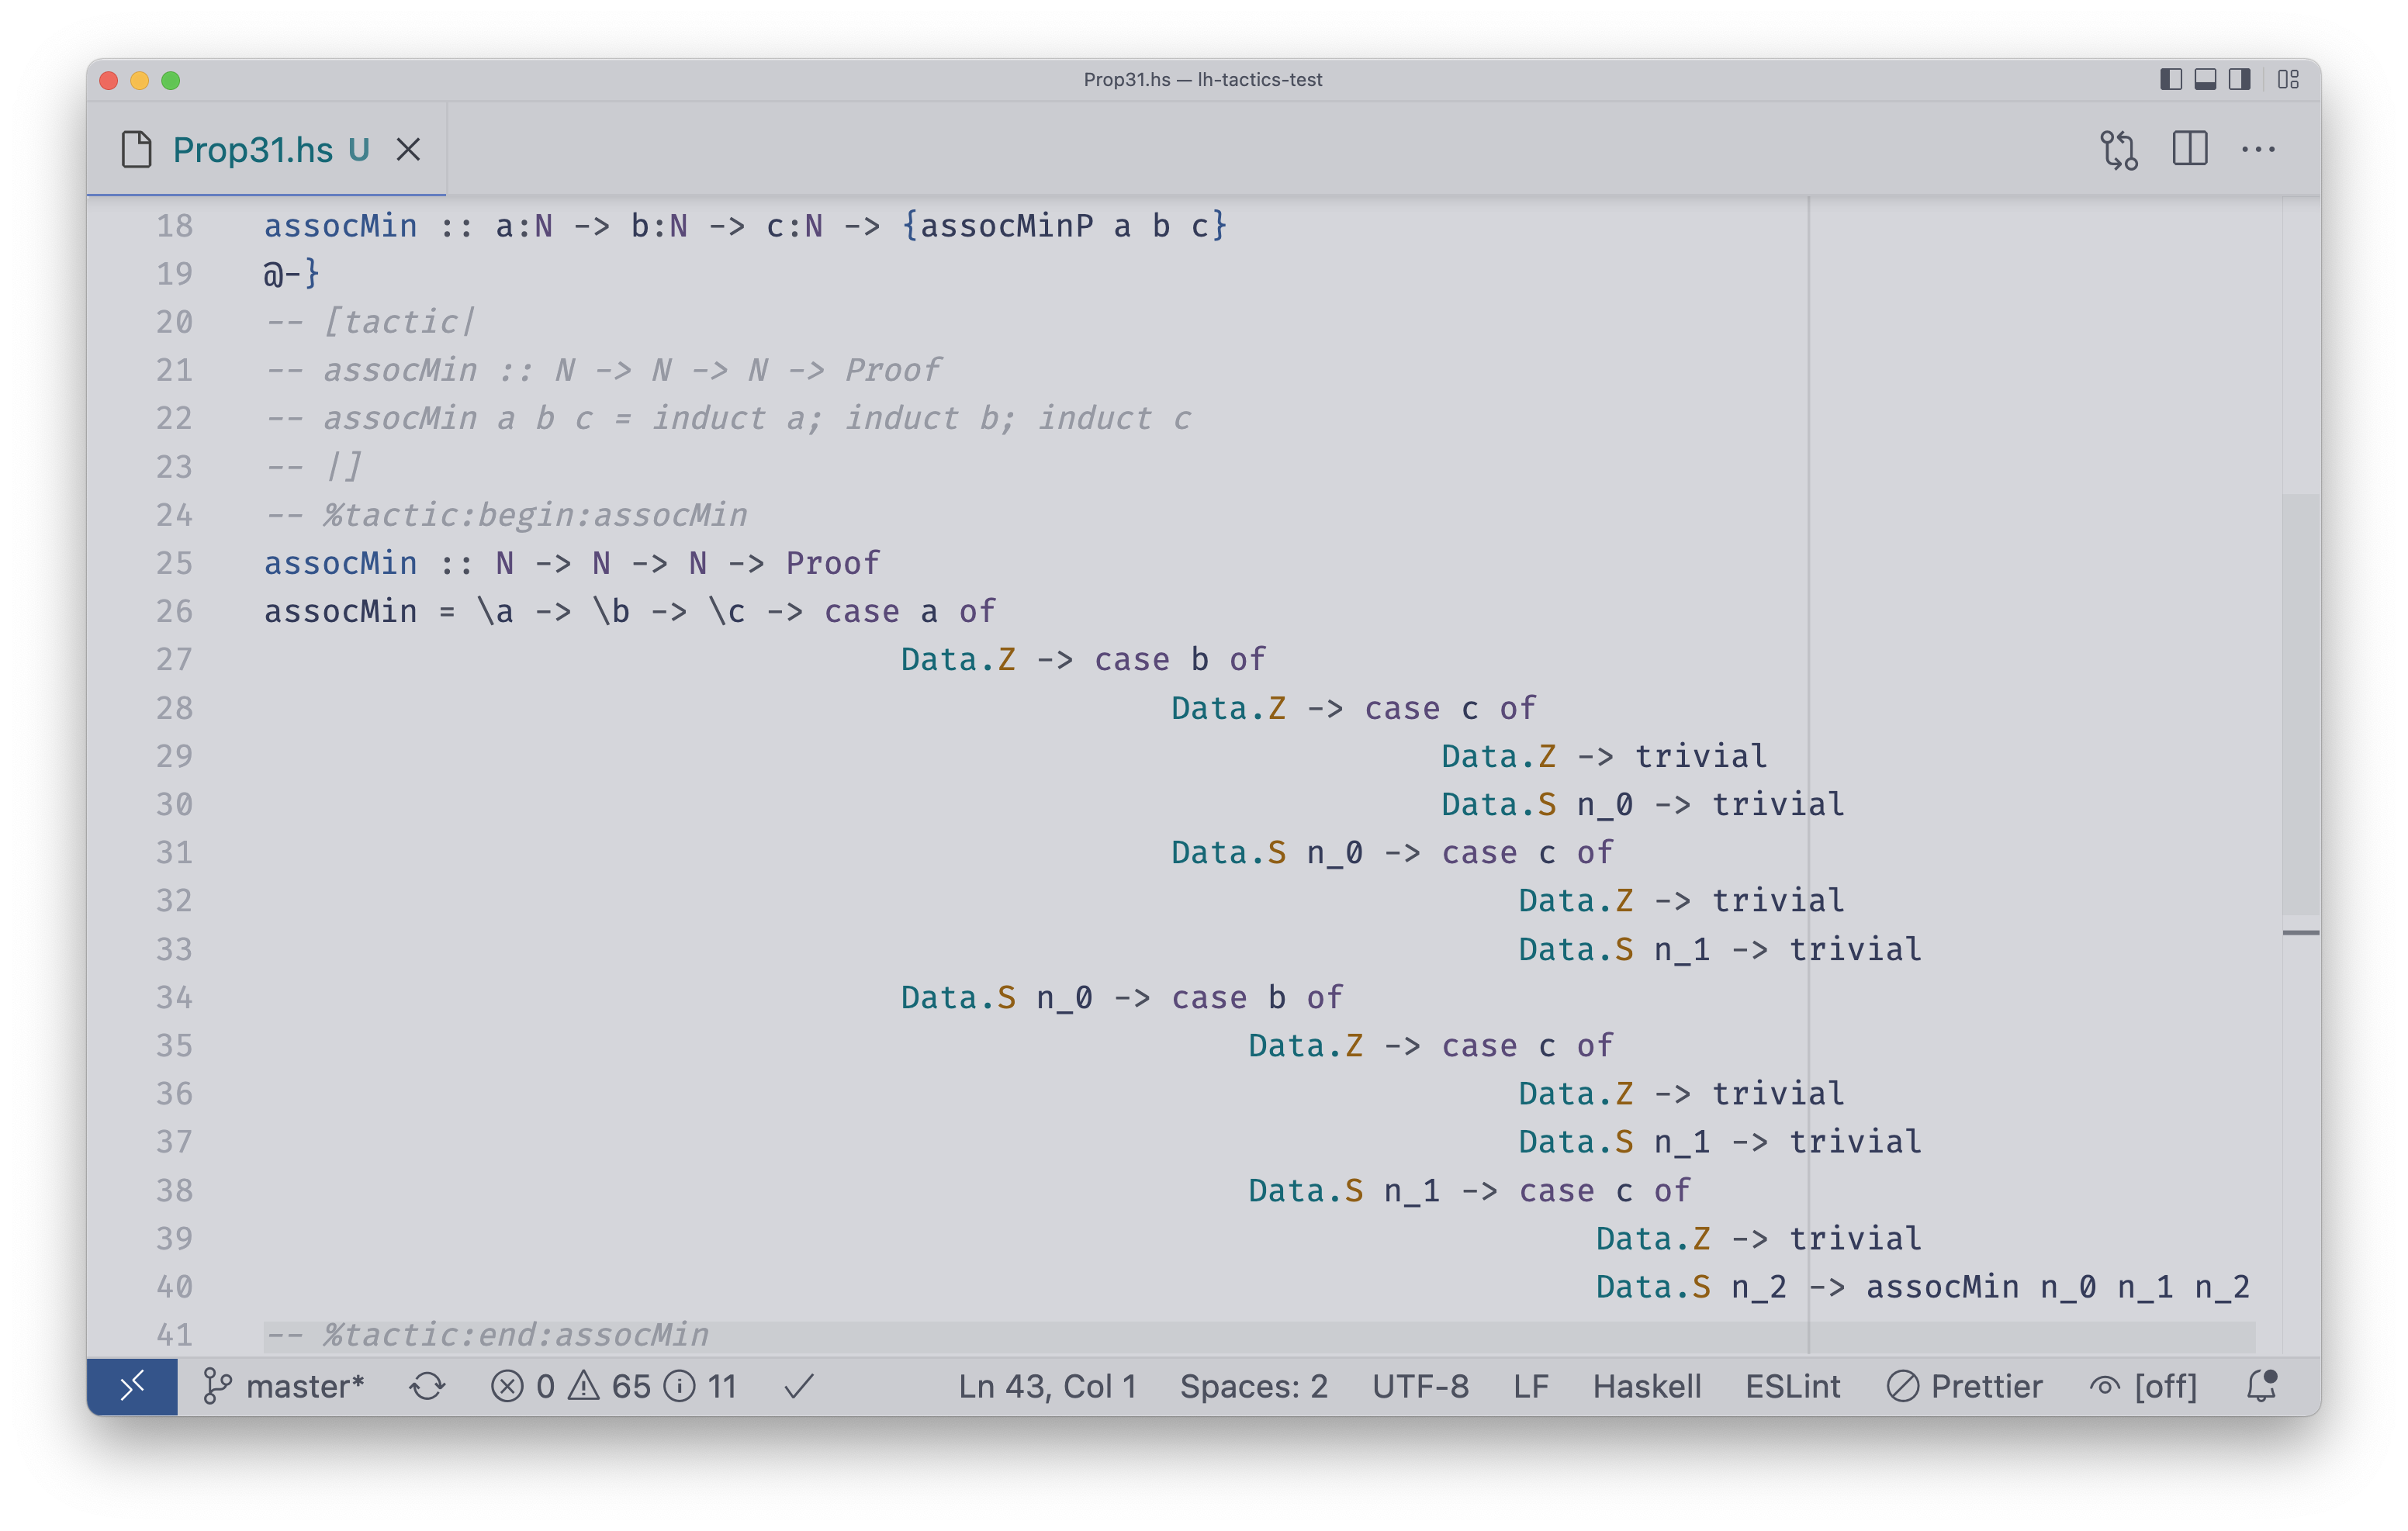
\includegraphics[width=\textwidth]{example-screenshots/done.png}
    \end{minipage}
    \hfill
    \begin{minipage}[c]{0.3\textwidth}
      \caption{Once pruning has completed, the final proof term is presented and
      the original proof macros that generated it are left in a comment 
      immediately above.}    \end{minipage}
  \end{subfigure}
  % &
  % \begin{subfigure}[t][][t]{1\textwidth}
  %   \centering
  %   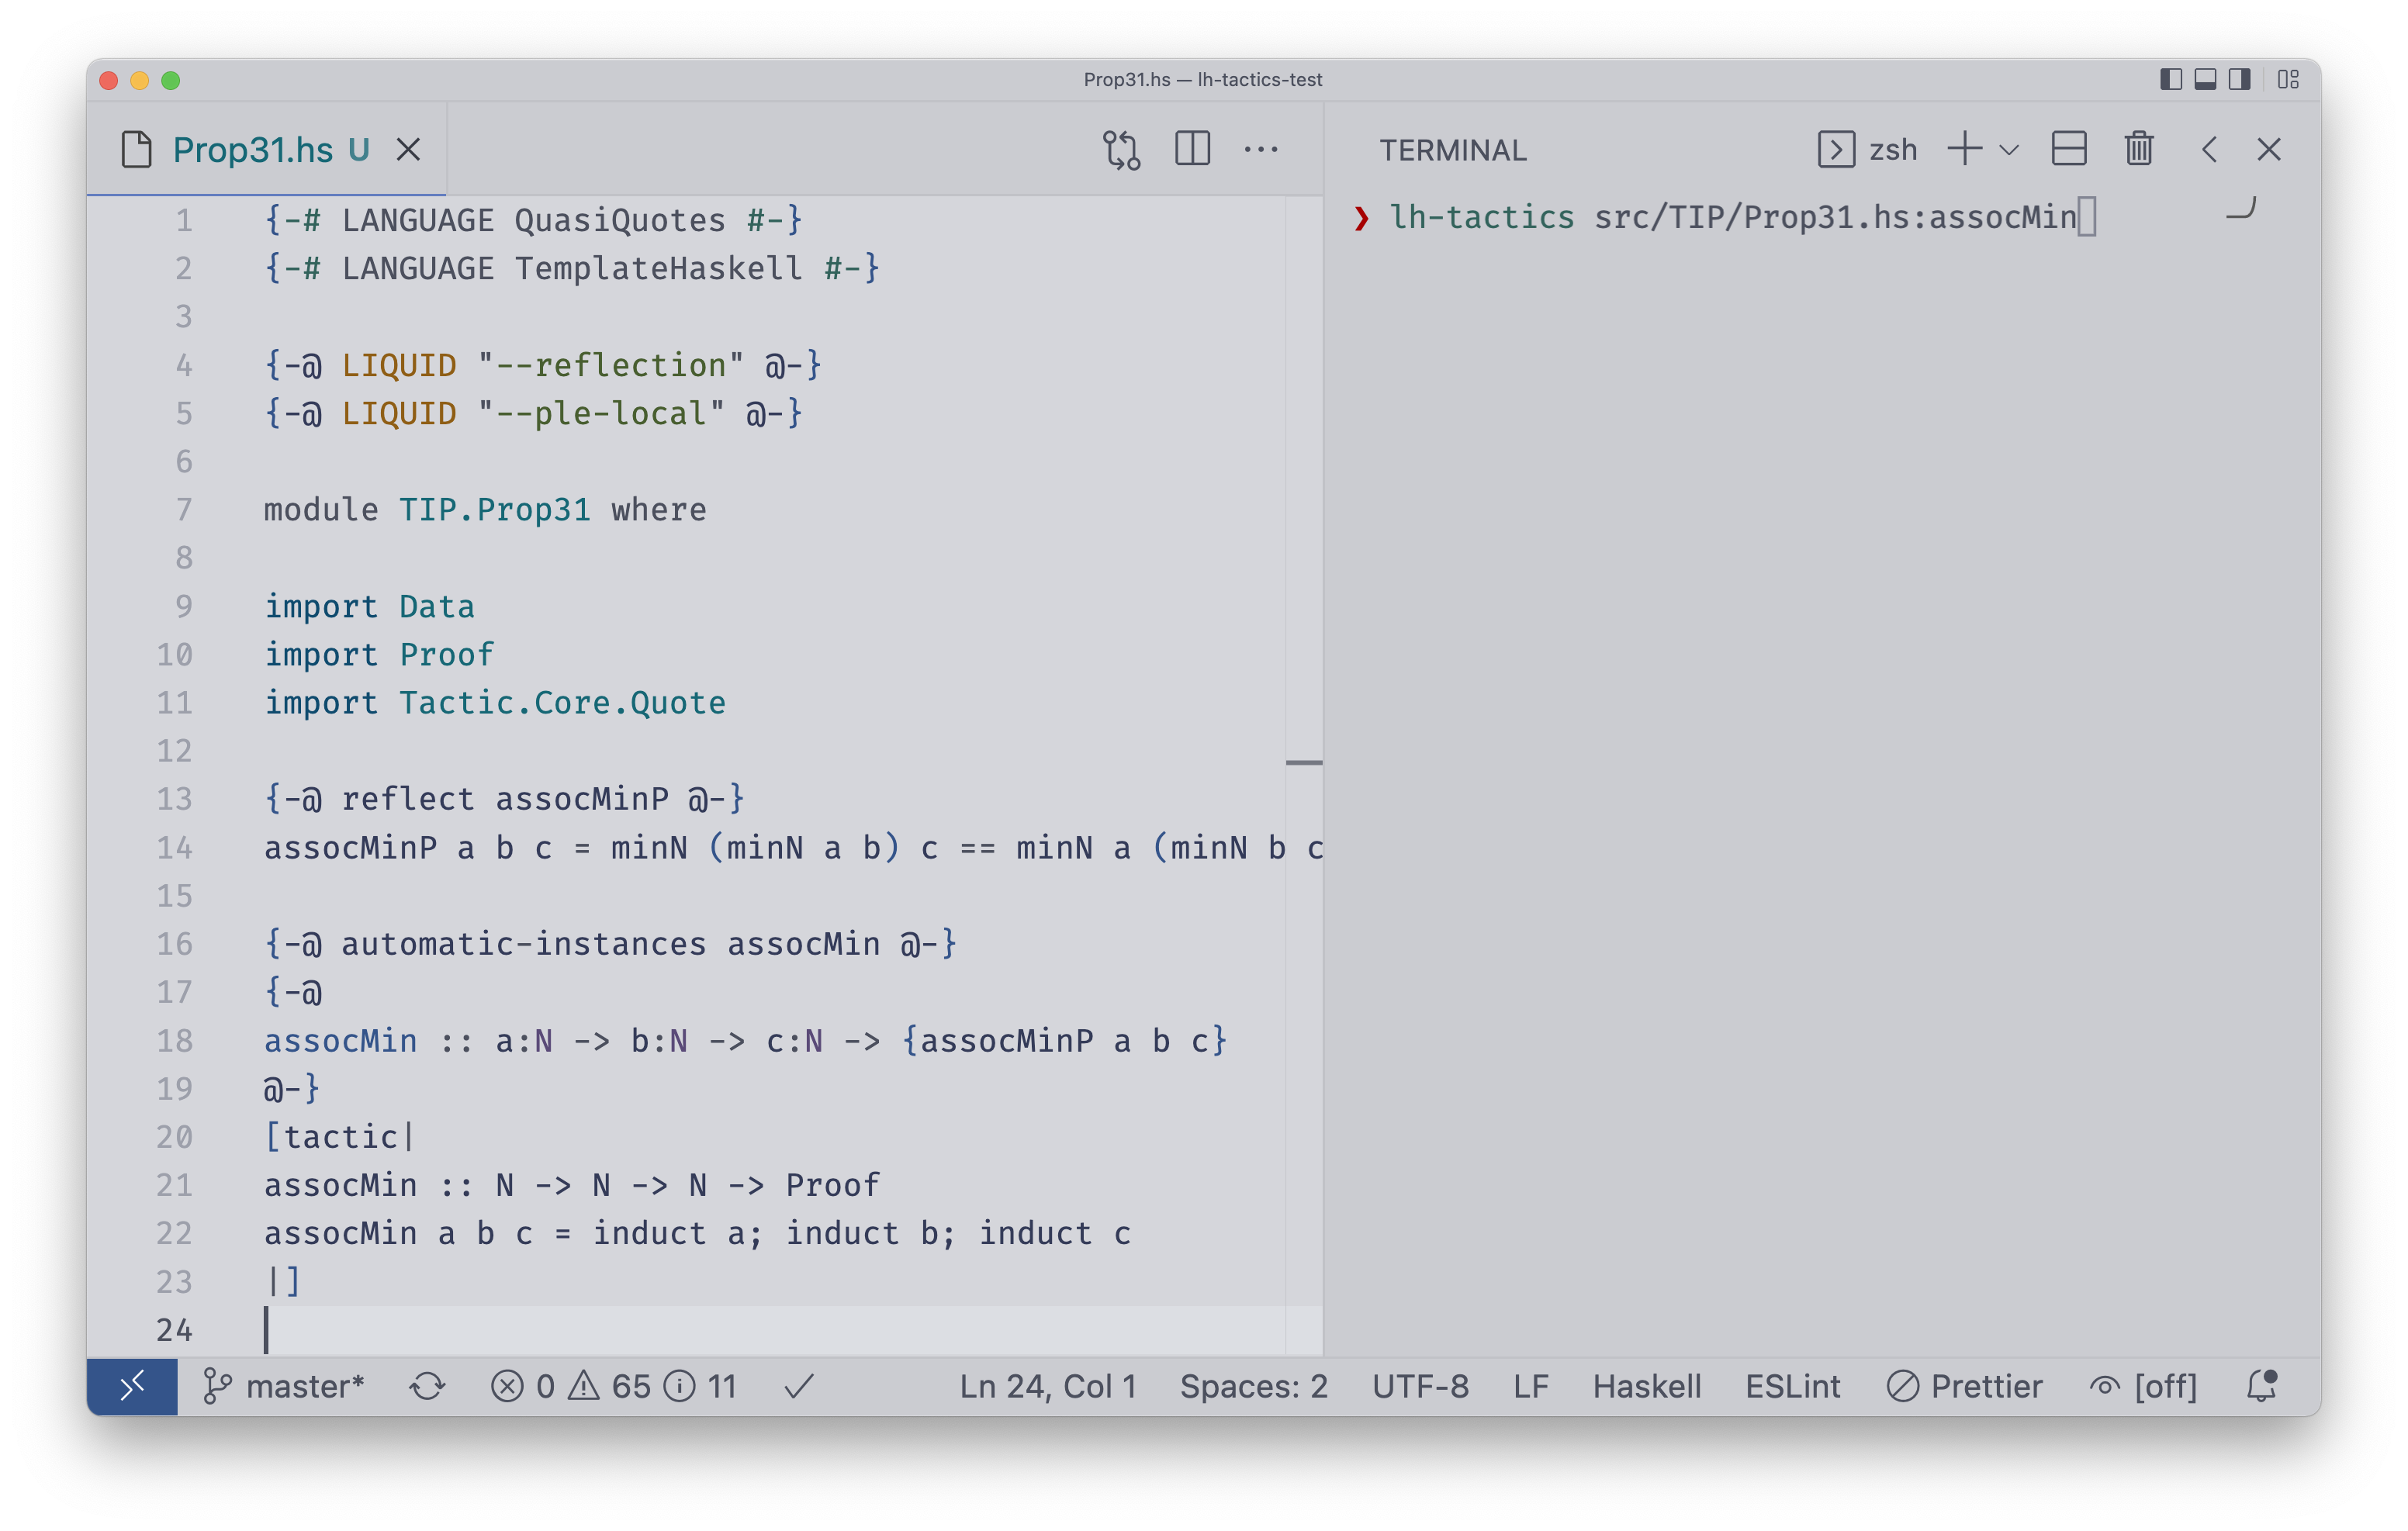
\includegraphics[width=\textwidth]{example-screenshots/run.png}
  %   \caption{The user runs the \LC{lh-tactics} command line tool on the input
  %   file, which exists inside of a \textit{stack} project that is configured to
  %   use the LiquidHaskell as a plugin.}
  % \end{subfigure}
  % % \\
  % \begin{subfigure}[t][][t]{1\textwidth}
  %   \centering
  %   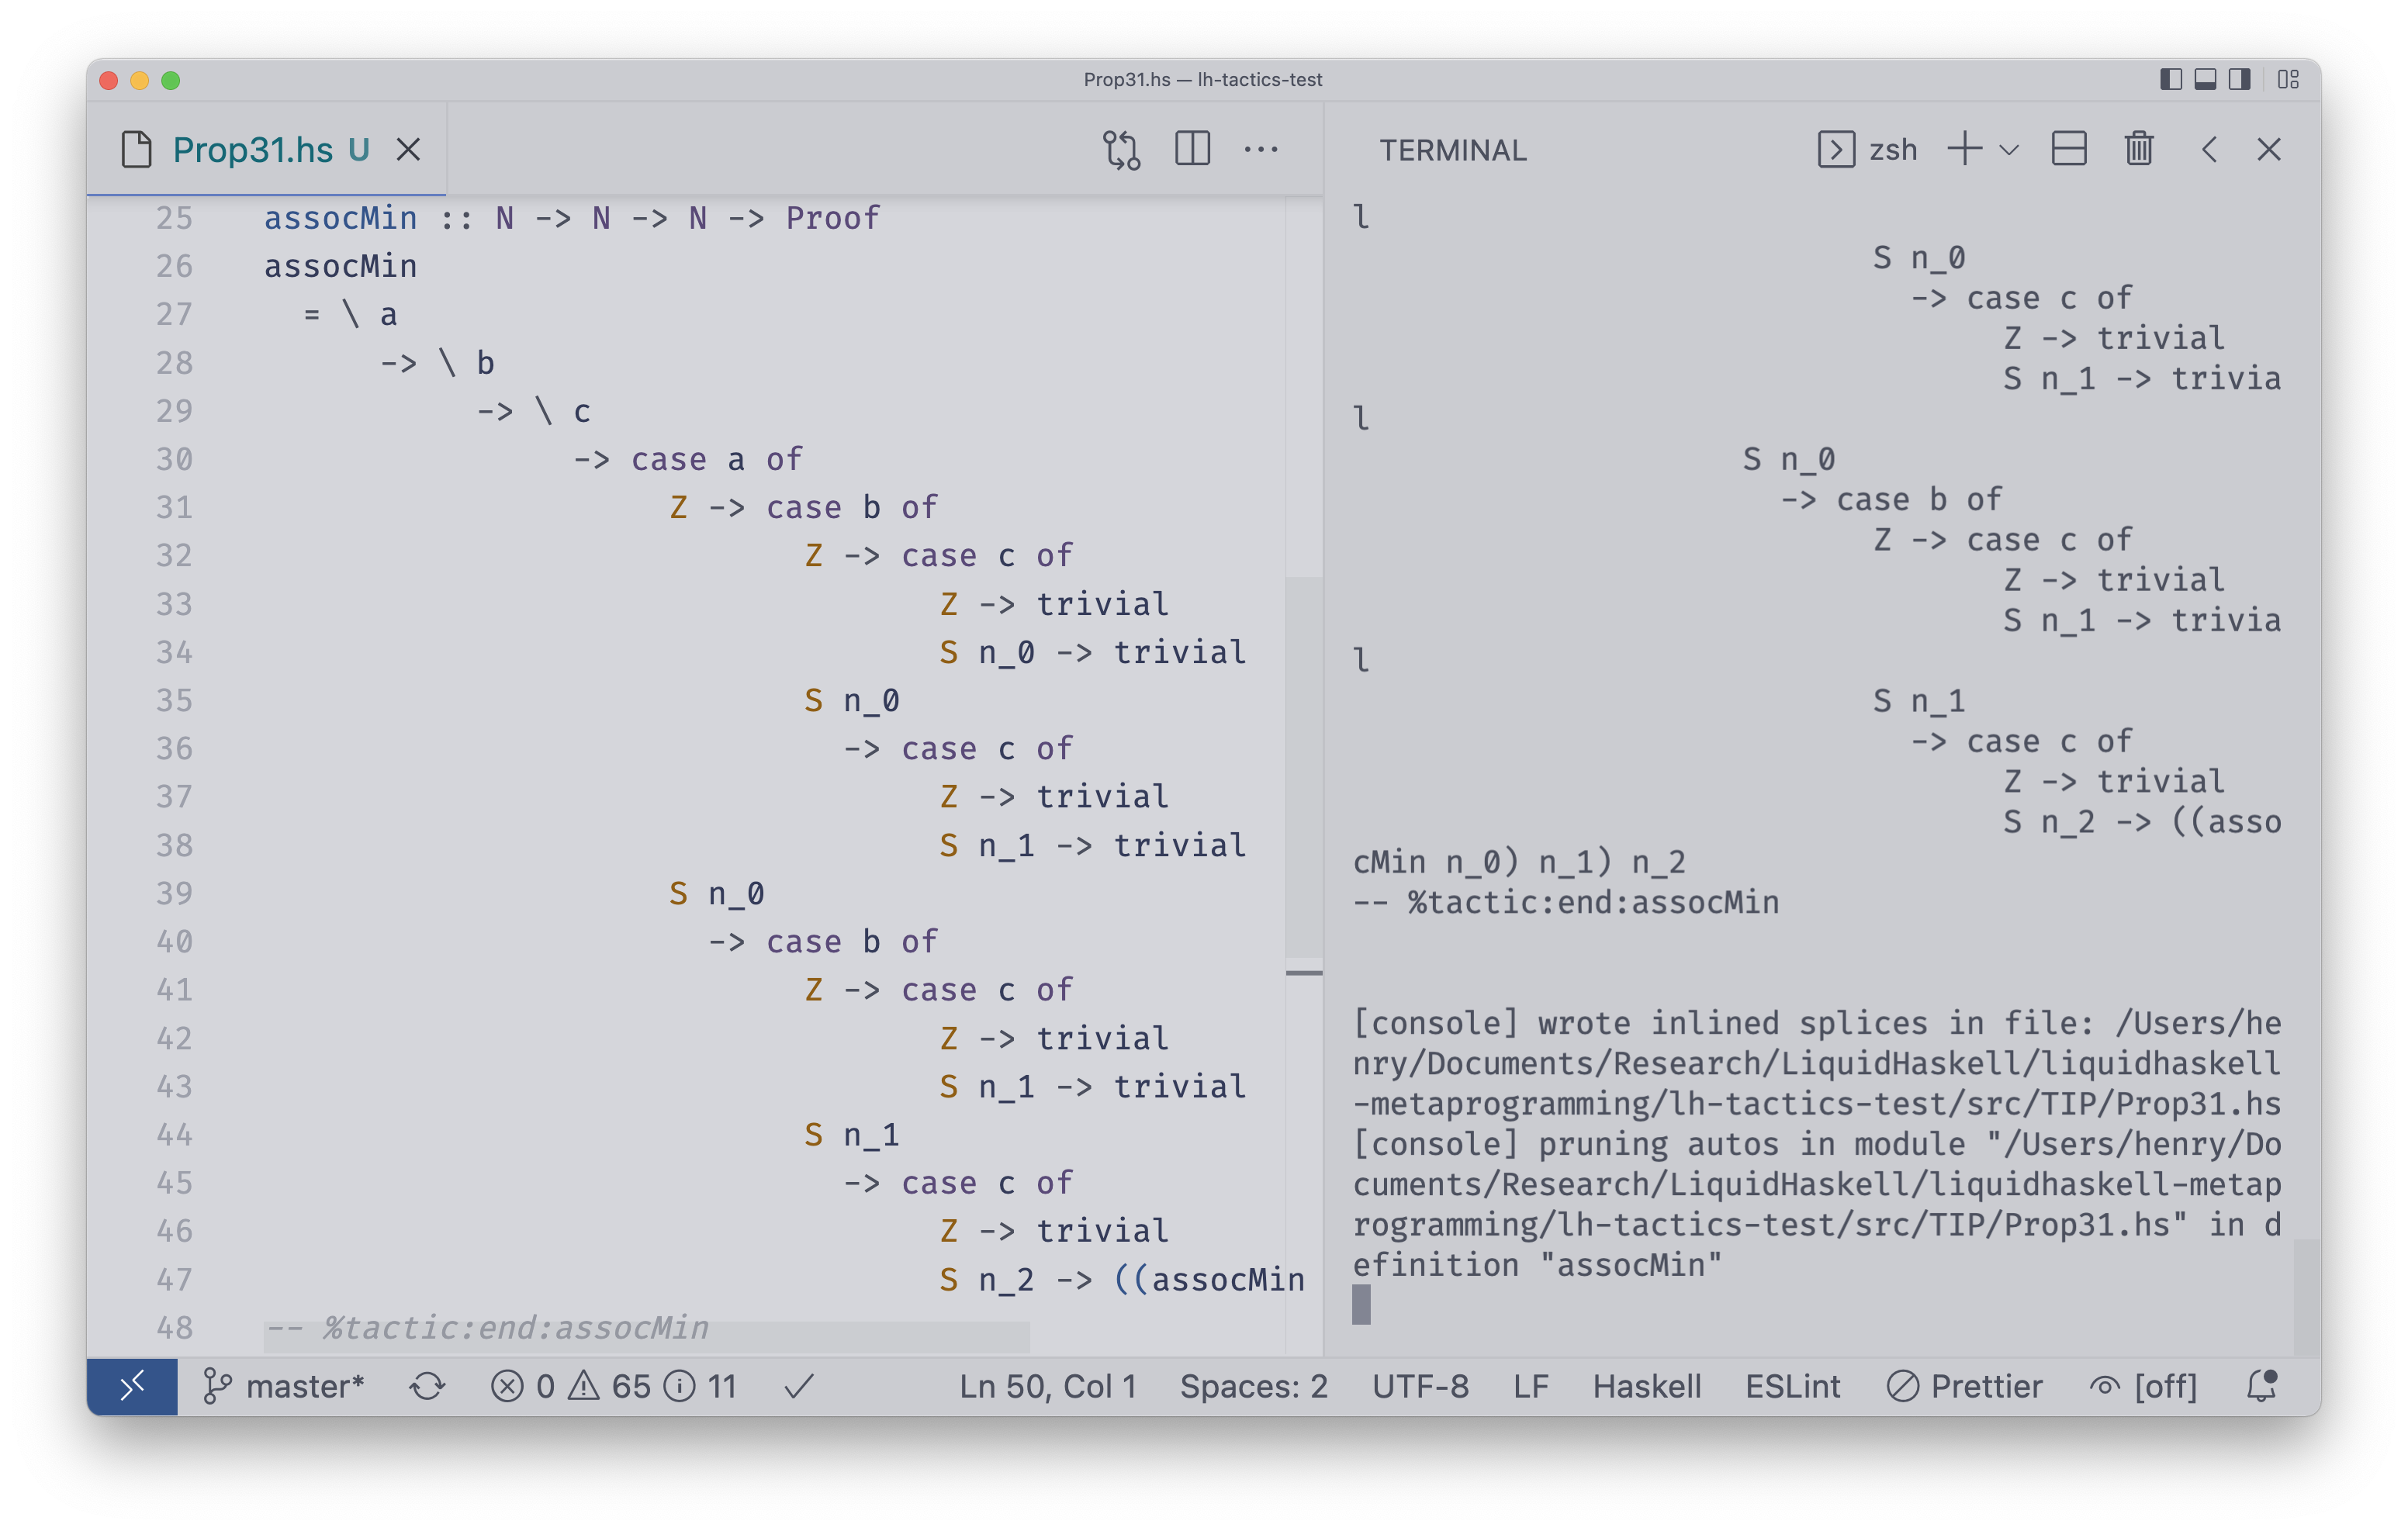
\includegraphics[width=\textwidth]{example-screenshots/pruning.png}
  %   \caption{The user waits for the \LC{lh-tactics} tool to complete. During
  %   this time, the tool will overwrite the input file on each pruning attempt.}
  % \end{subfigure}
  % % &
  % \begin{subfigure}[t][][t]{1\textwidth}
  %   \centering
  %   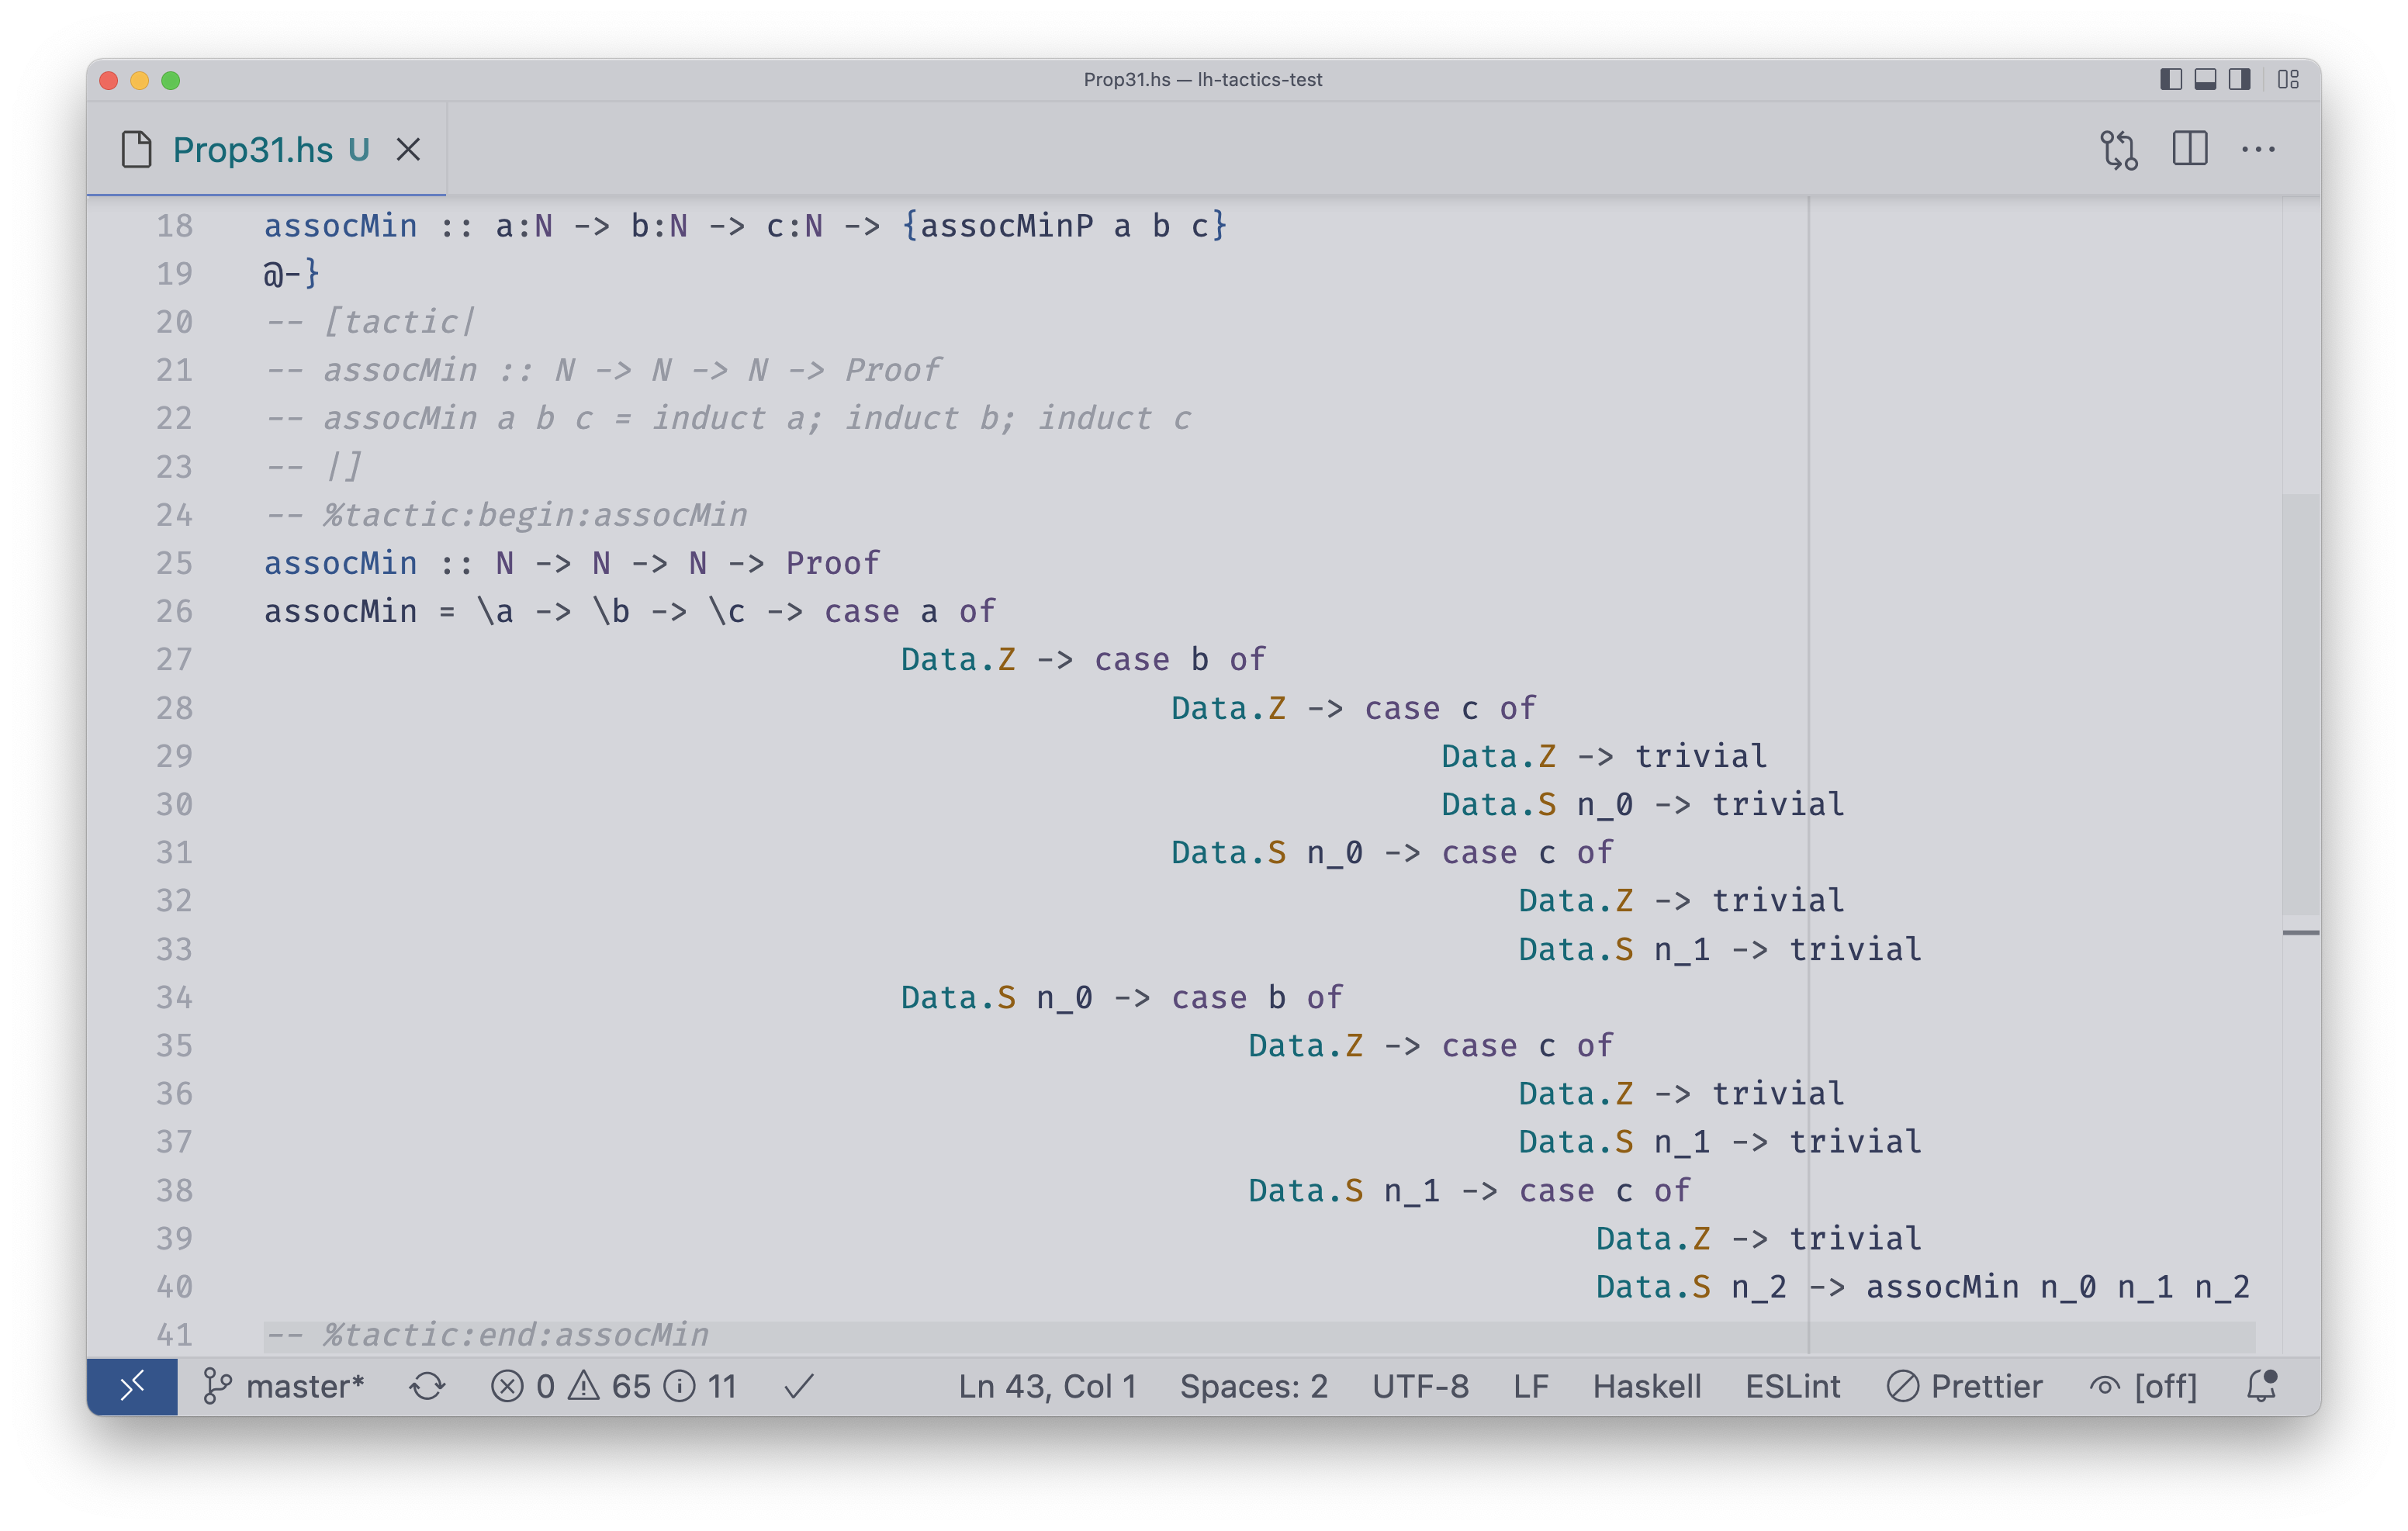
\includegraphics[width=\textwidth]{example-screenshots/done.png}
  %   \caption{Once pruning has completed, the final proof term is presented and
  %   the original proof macros that generated it are left in a comment 
  %   immediately above.}
  % \end{subfigure}

  % \begin{tabular}{cc}
  %   \begin{subfigure}[t][][t]{0.49\textwidth}
  %     \centering
  %     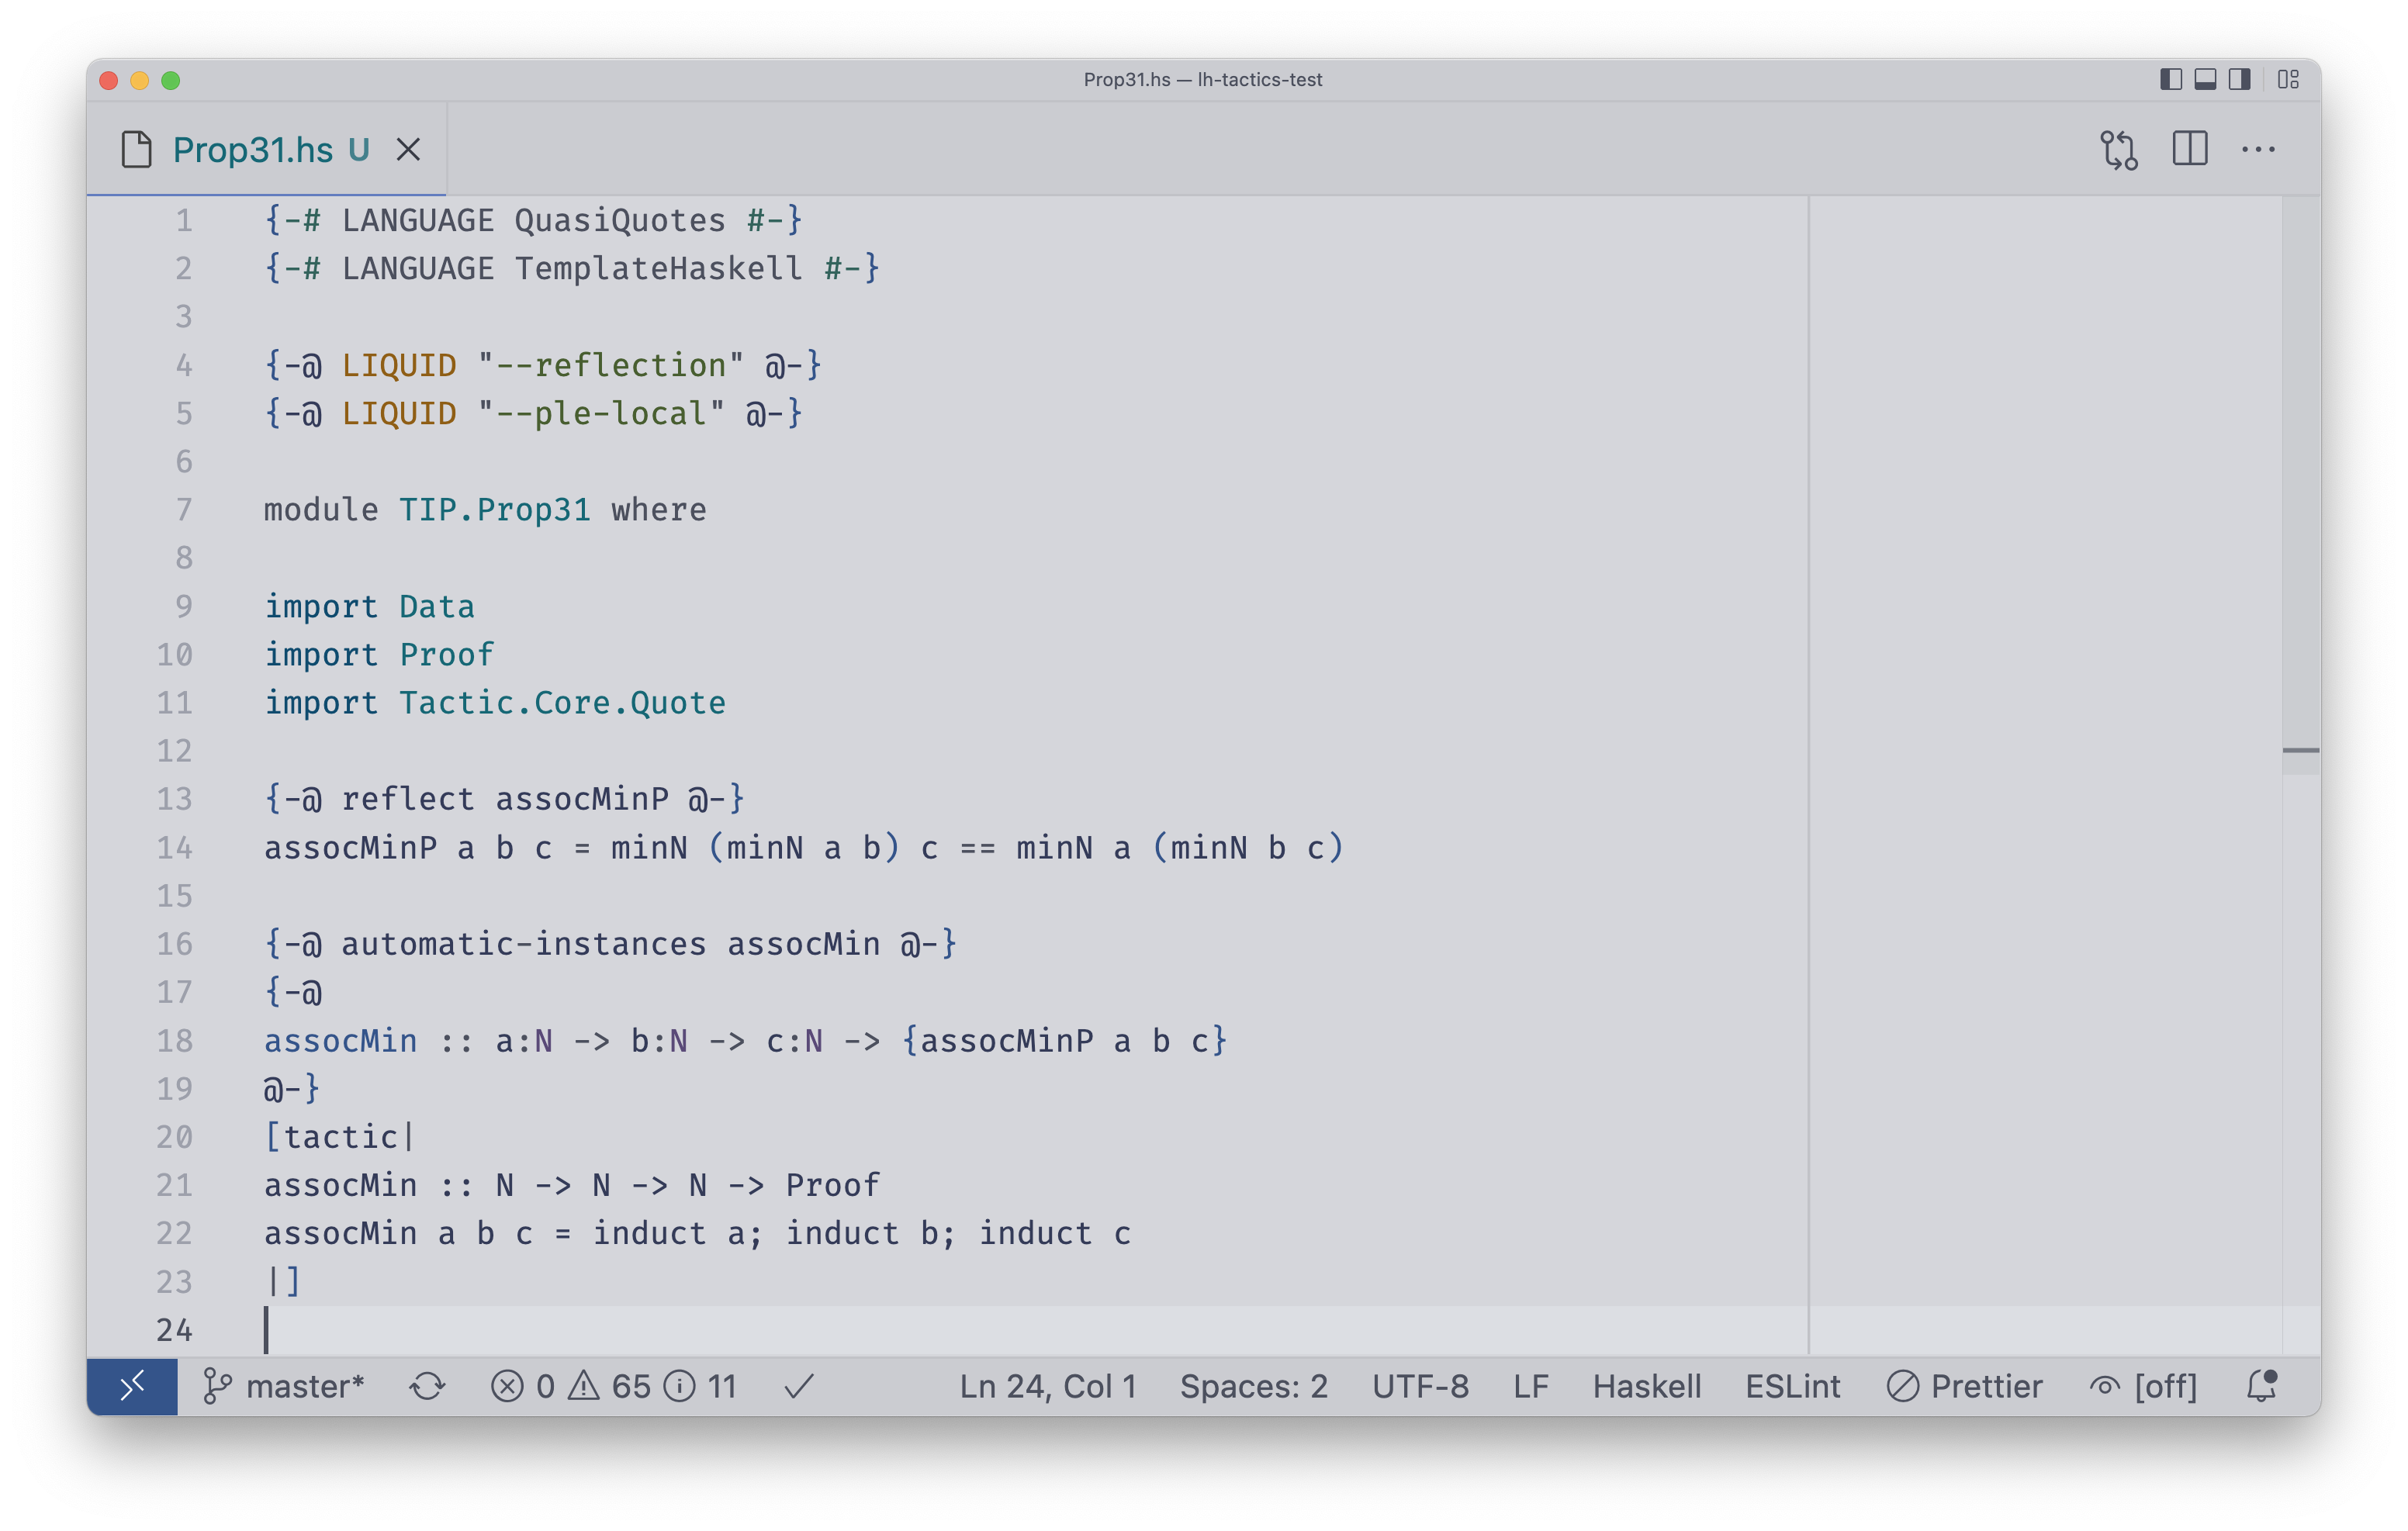
\includegraphics[width=\textwidth]{example-screenshots/macros.png}
  %     \caption{The user writes the proof macros.}
  %   \end{subfigure}
  %   &
  %   \begin{subfigure}[t][][t]{0.49\textwidth}
  %     \centering
  %     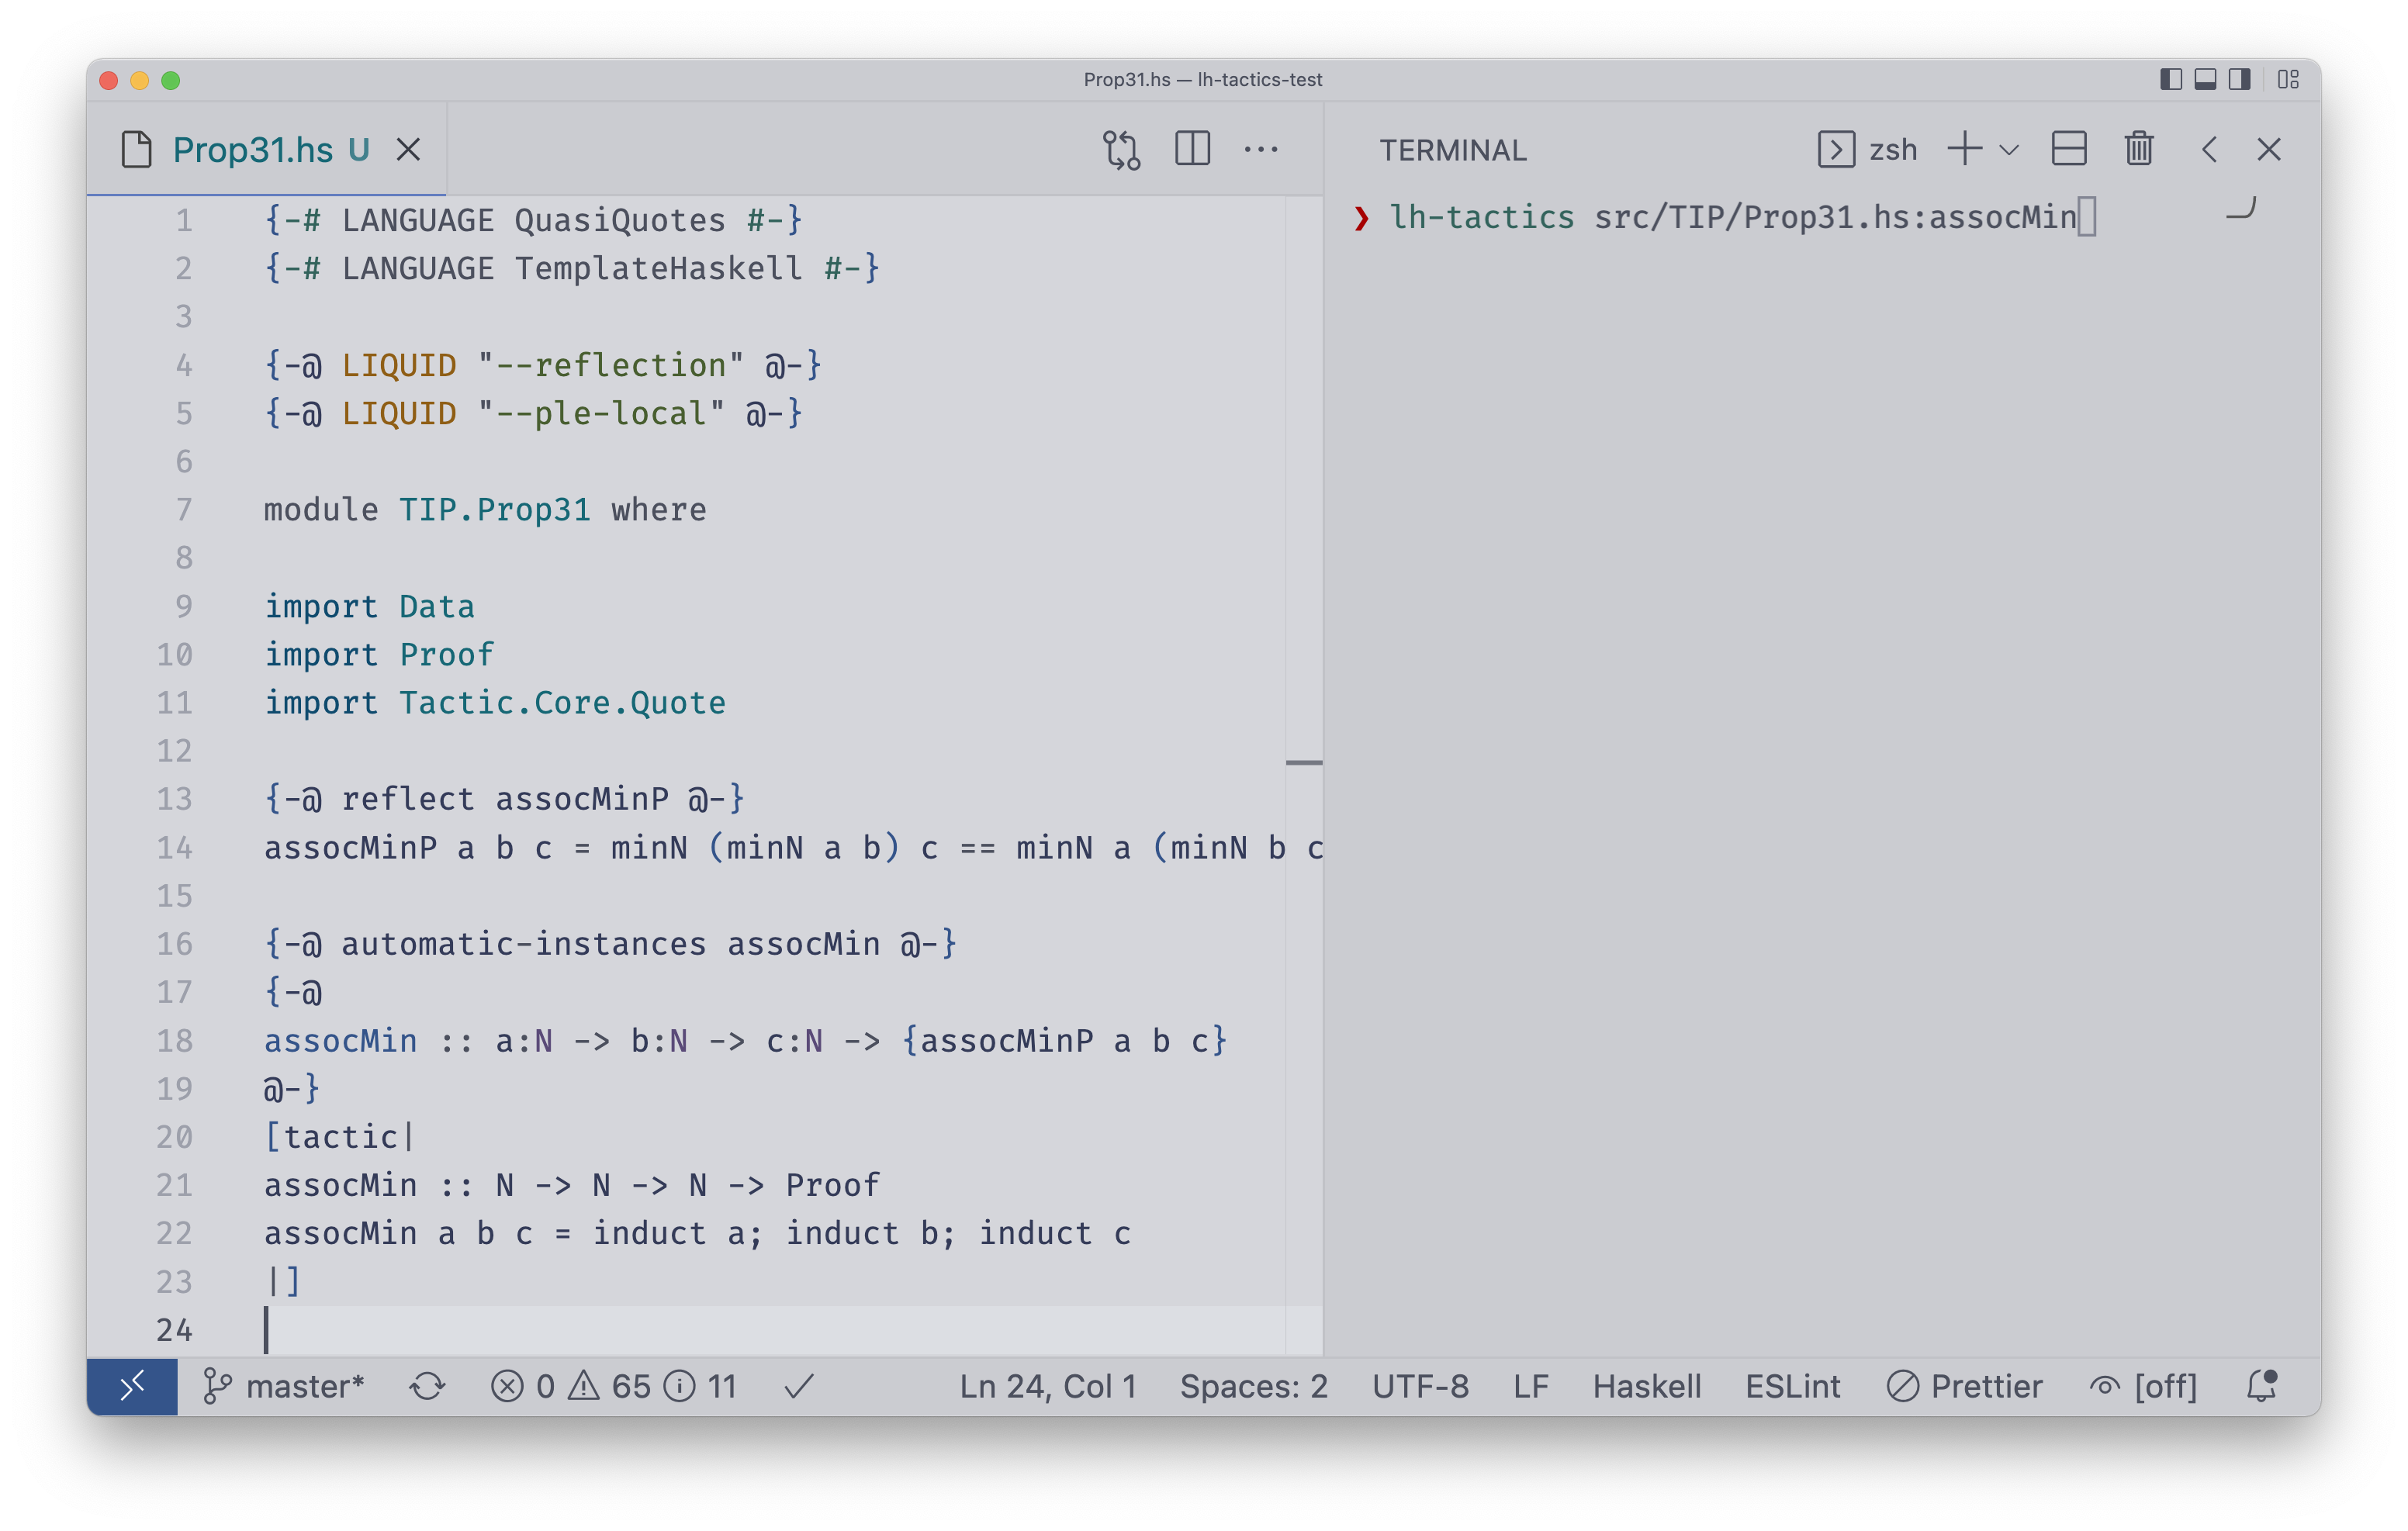
\includegraphics[width=\textwidth]{example-screenshots/run.png}
  %     \caption{The user runs the \LC{lh-tactics} command line tool on the input
  %     file, which exists inside of a \textit{stack} project that is configured to
  %     use the LiquidHaskell as a plugin.}
  %   \end{subfigure}
  %   \\
  %   \begin{subfigure}[t][][t]{0.49\textwidth}
  %     \centering
  %     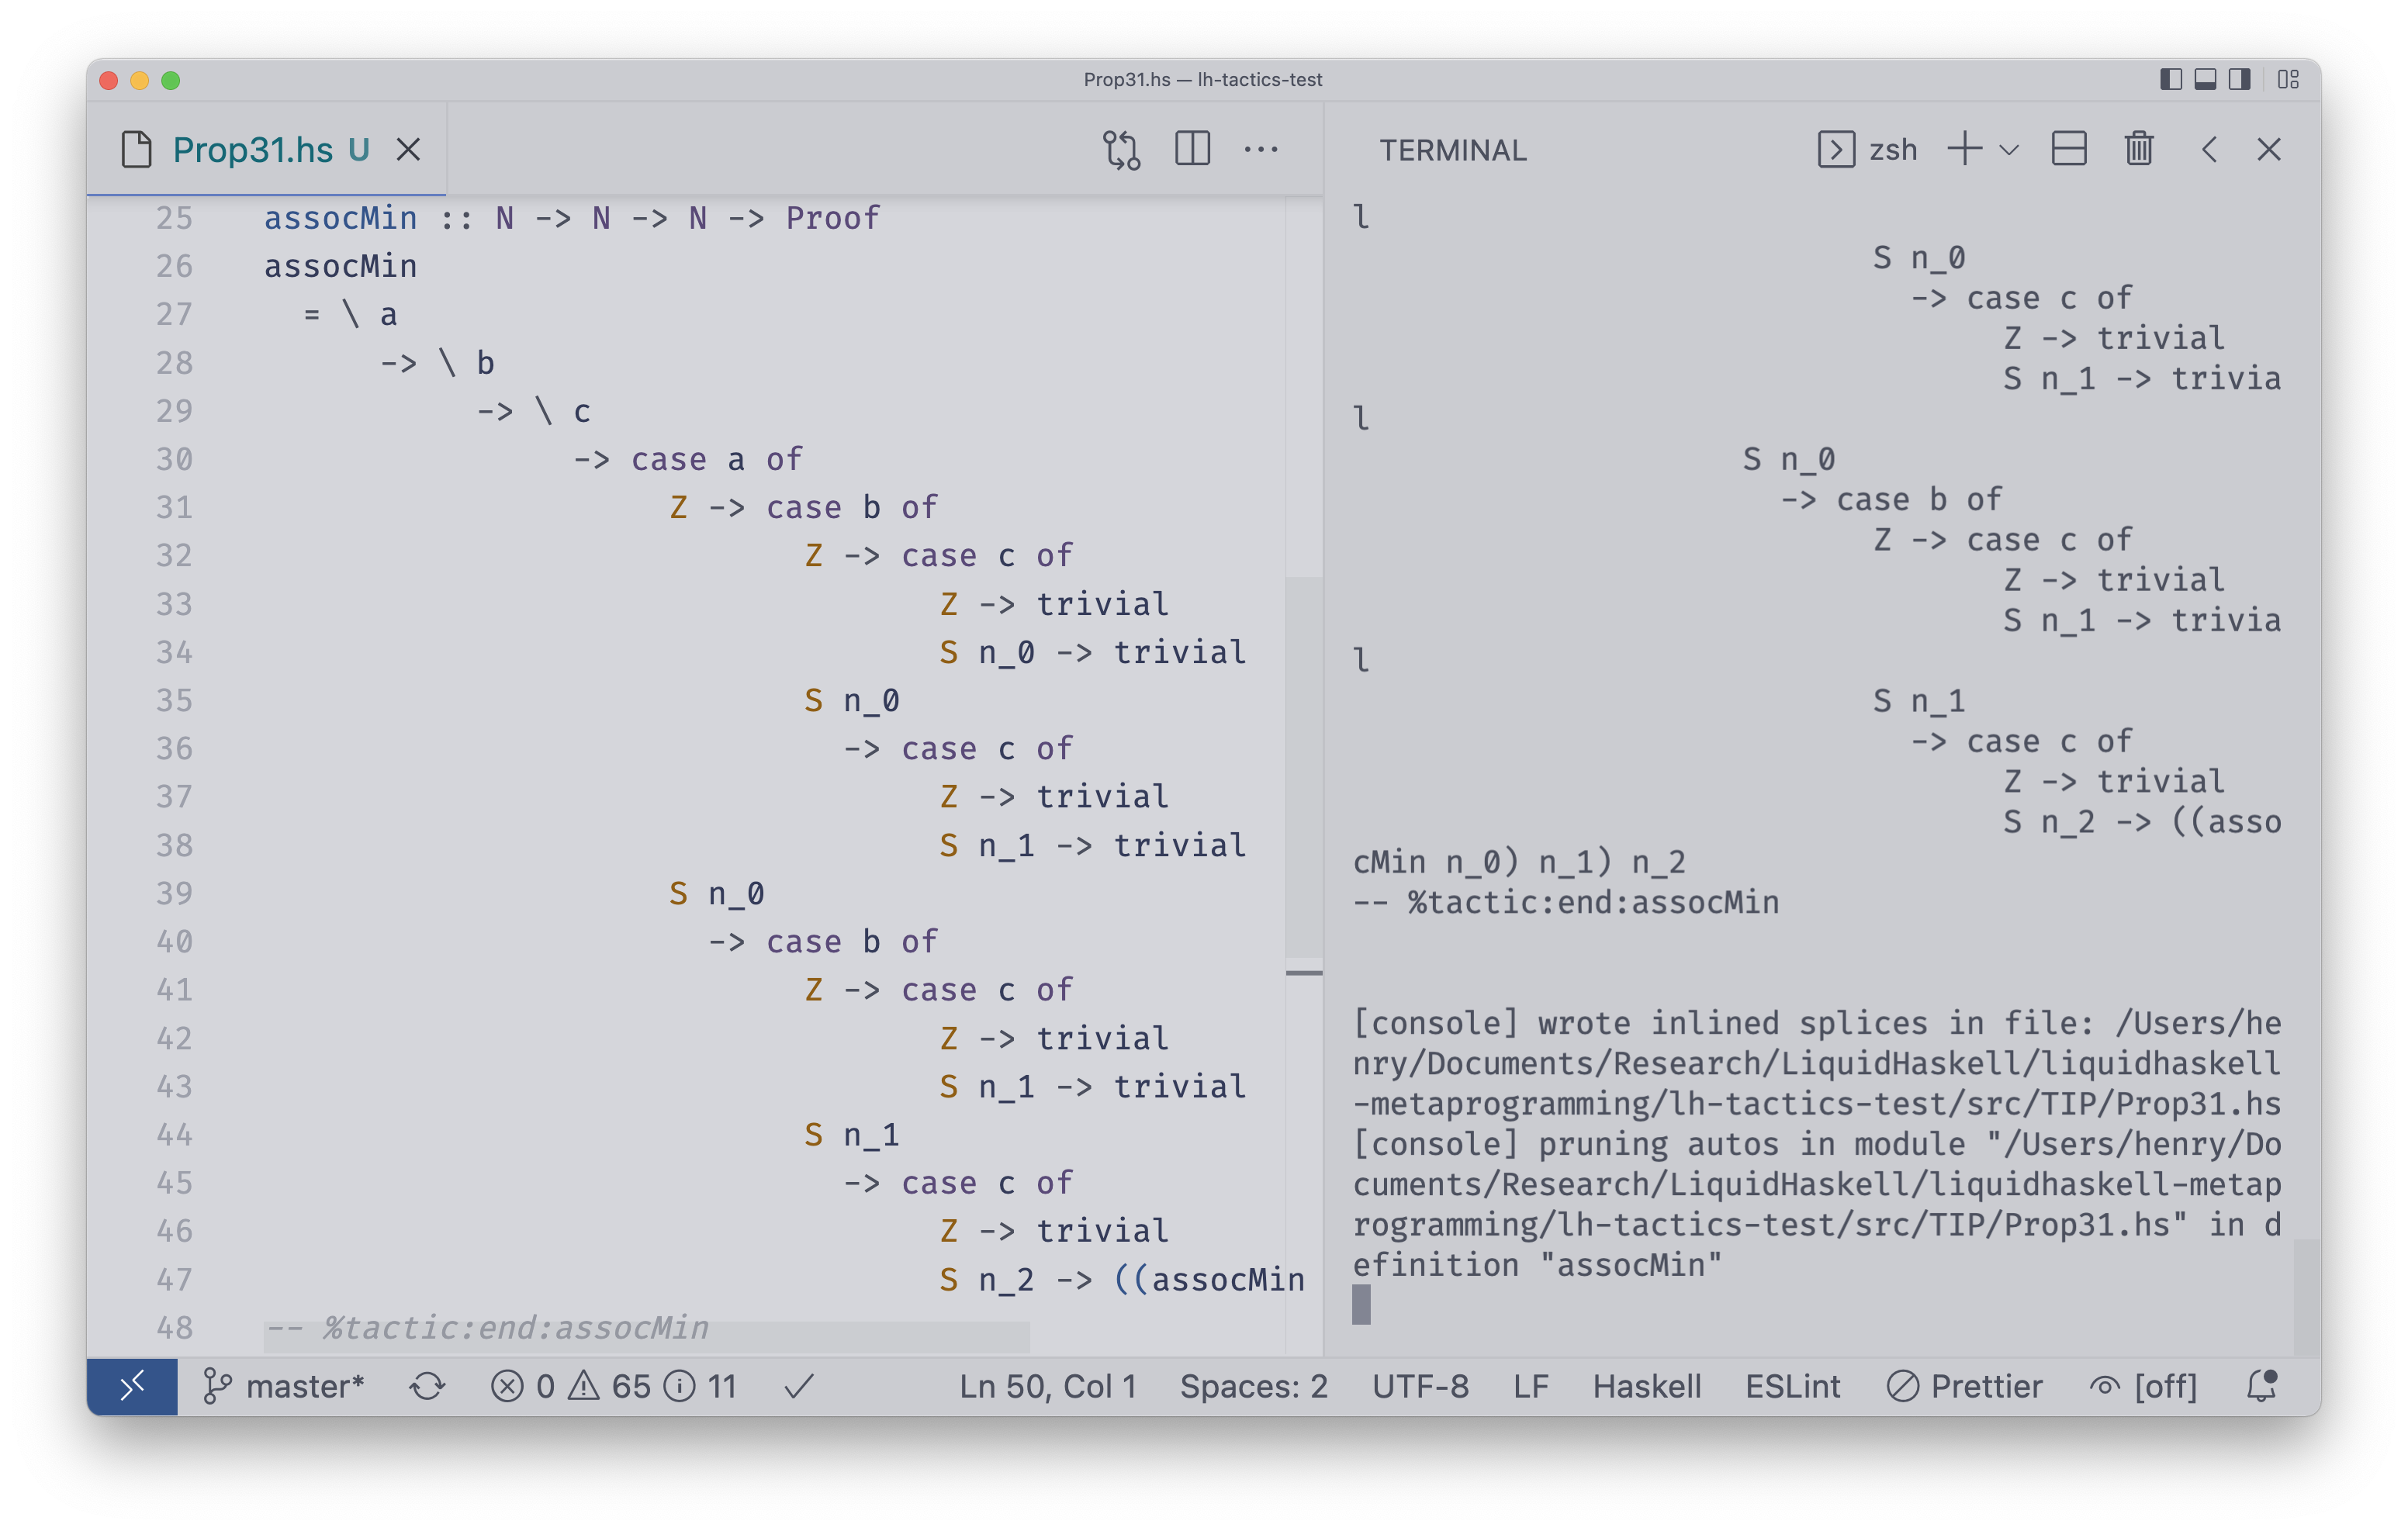
\includegraphics[width=\textwidth]{example-screenshots/pruning.png}
  %     \caption{The user waits for the \LC{lh-tactics} tool to complete. During
  %     this time, the tool will overwrite the input file on each pruning attempt.}
  %   \end{subfigure}
  %   &
  %   \begin{subfigure}[t][][t]{0.49\textwidth}
  %     \centering
  %     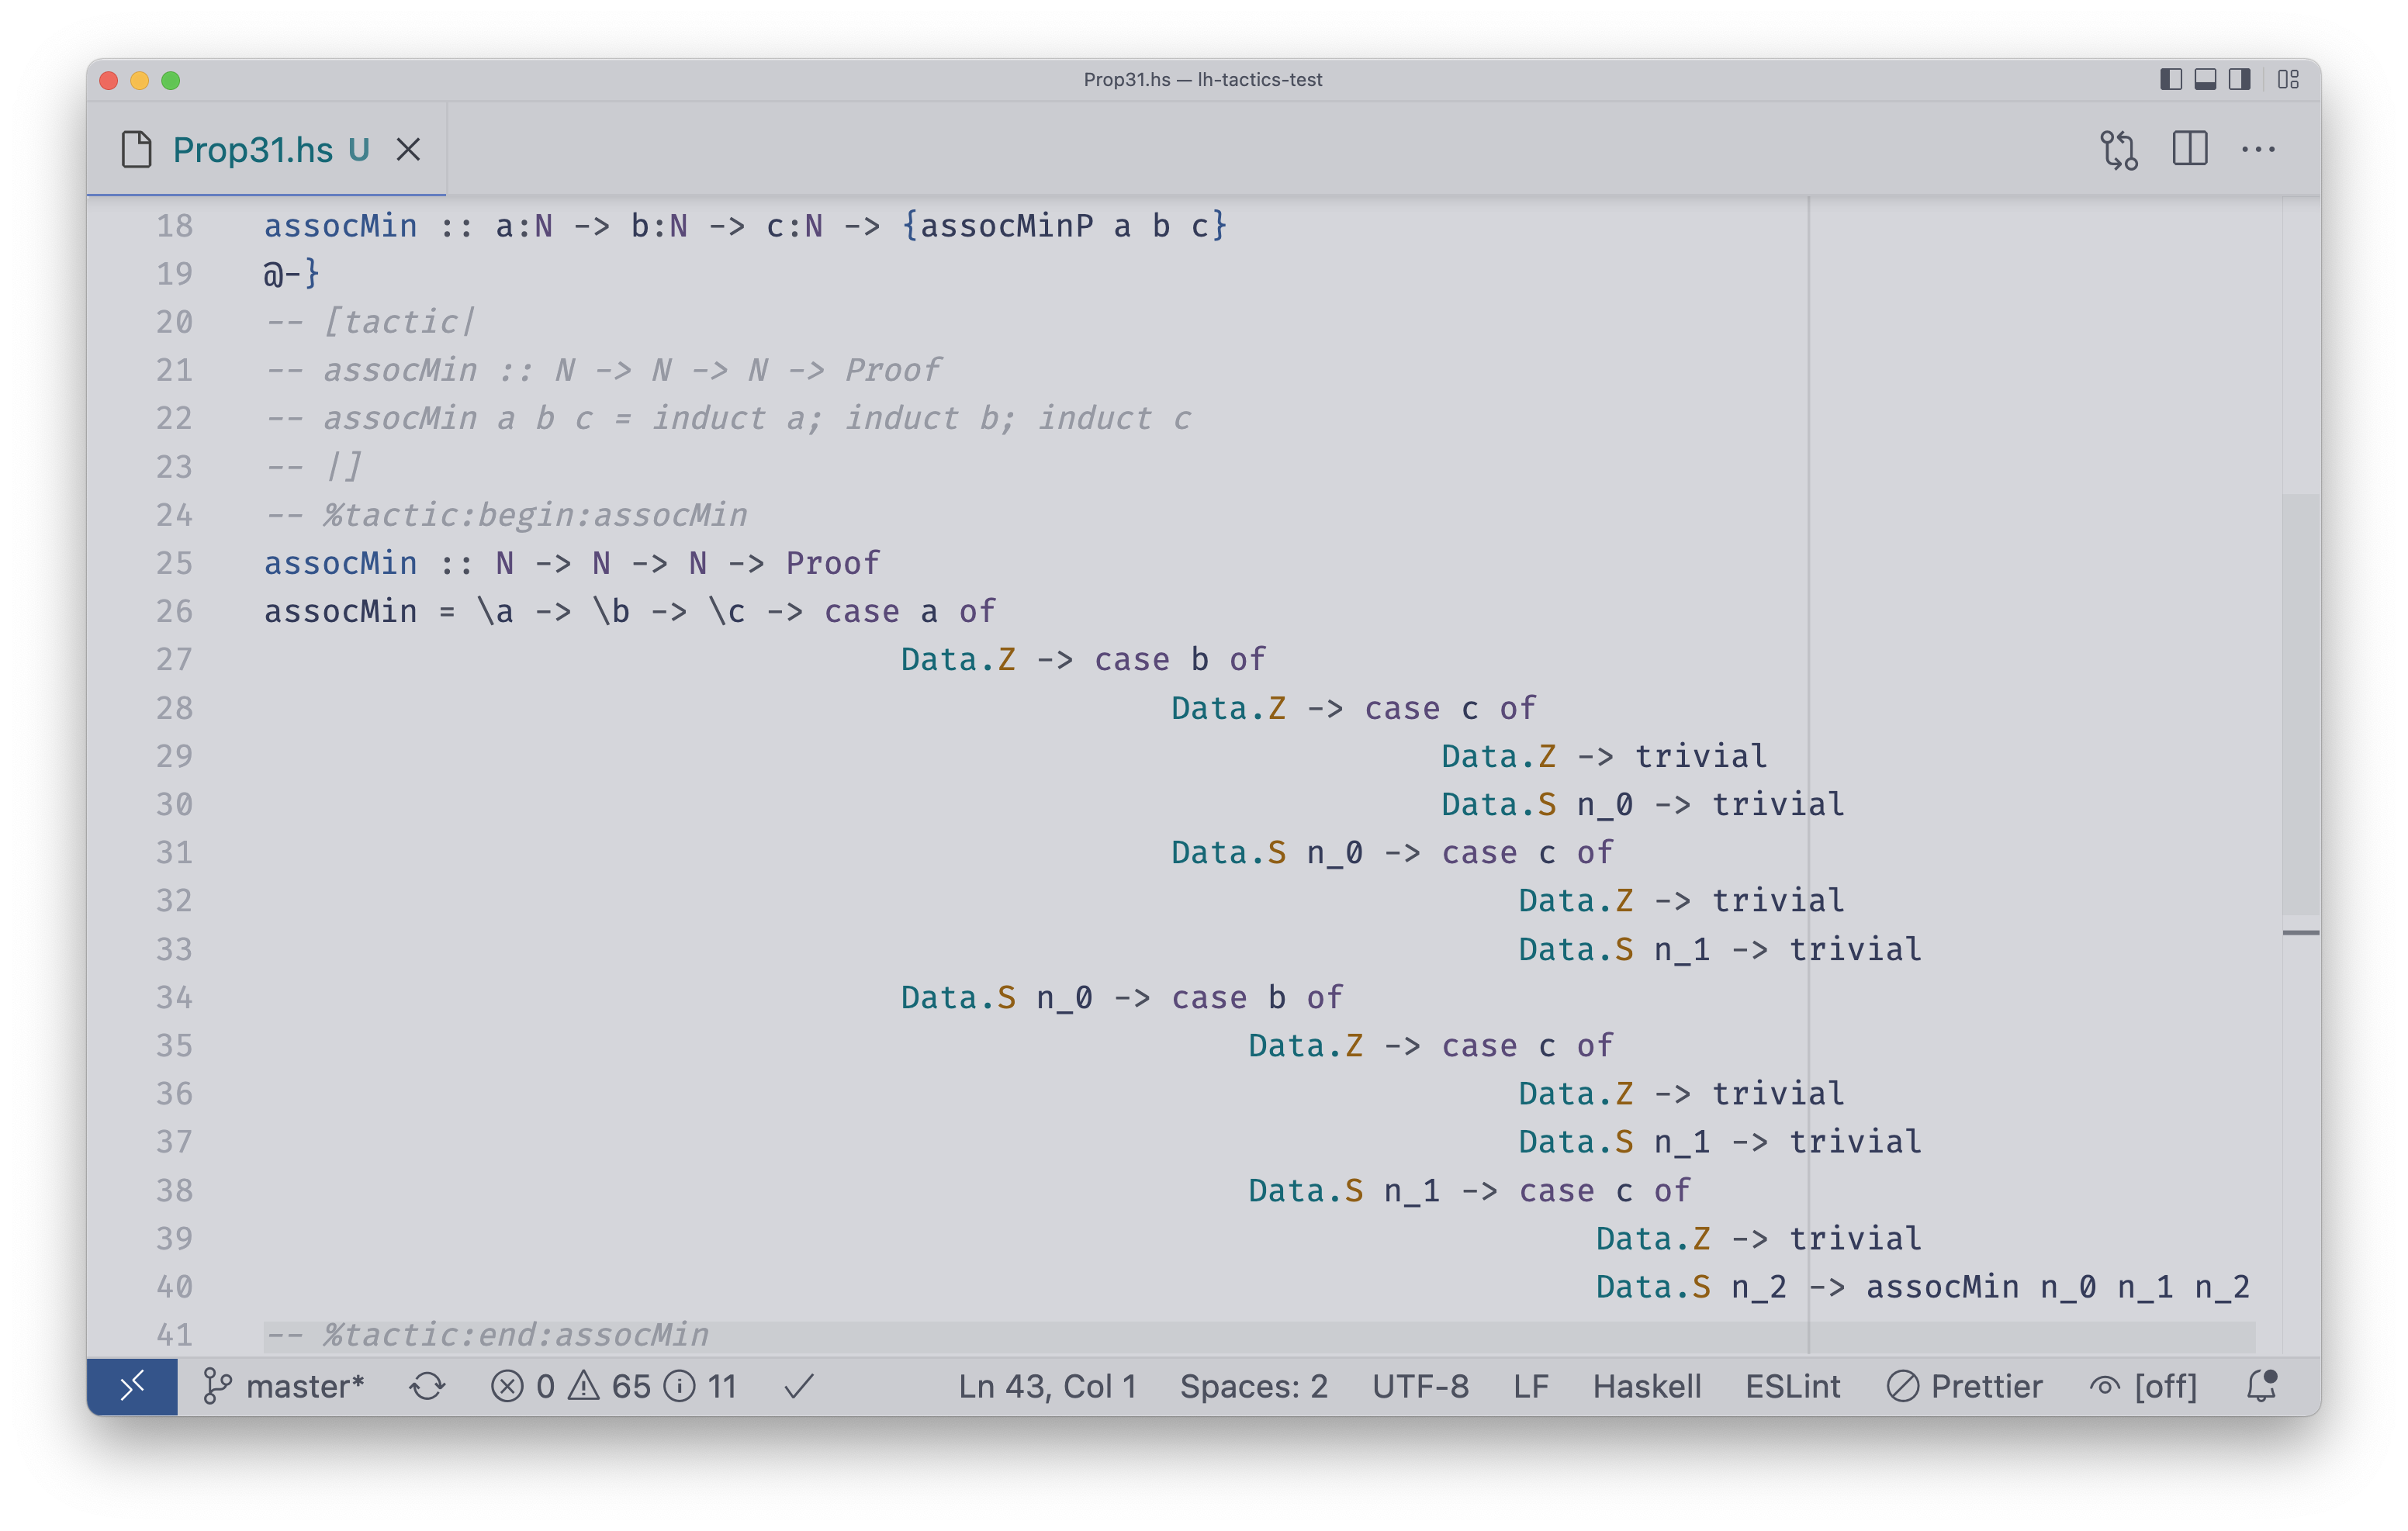
\includegraphics[width=\textwidth]{example-screenshots/done.png}
  %     \caption{Once pruning has completed, the final proof term is presented and
  %     the original proof macros that generated it are left in a comment 
  %     immediately above.}
  %   \end{subfigure}
  % \end{tabular}
  
  % \begin{minipage}{\textwidth}
  % \end{minipage}
  \caption{Usage example of the proof macros tool.}
  \label{fig:usage}
\end{figure*}

\subsection{Usage Example}
\label{sec:example}

Figure~\ref{fig:usage} shows the user's workflow when proving a
theorem such as \LC{assocMin} from the introduction
(Figure~\ref{fig:assoc-min-macro}). It shows three screenshots of
VSCode with proof macro processing in progress. First, the user must
invoke our tool \LC{lh-tactics}, which then parses the proof macro,
expands it, and repeatedly prunes it until a minimal proof term is
reached (see Figure~\ref{fig:assoc-min-proof}).

% TODO: put screenshots here


%  
% \todo{format data better}
% \begin{figure*}
%   \begin{tabular}{ll}
%     \hline
%     Measure label & Measure value
%     \\ \hline
%     Number of inductive proof & 
%       66
%     \\
%     Number of inductive proofs solved by simple macros &
%       45 (0.68 of inductive proofs)
%     \\
%     LOC increase after macro expansion & 
%       median: 7, mean: 15.77, std: 34.66 
%     \\ 
%     LOC increase after macro expansion and pruning & 
%       median: 2, mean: 2.61, std: 3.3
%     \\
%     Number of reasonably\footnote{\todo{Define this}} prune-able proofs &
%       73 (0.92 of proofs)
%     \\ \hline
%    \end{tabular}
%   \label{fig:evaluation}
% \end{figure*}

% \leo{Maybe some interesting examples here/outlier discussion?}
% \hen{I could include an example where the number of terms generated by auto was
% too large, so I had to manually provide lemma applications myself using the
% \macro{use} macro.
% Here's one below}
%  
% \begin{code}
%   {-@ sub_m_Sn ::  m:N -> n:N -> 
%         {subN m n == S (subN m (S n))} @-}
%  
%   {-@ sub_Sm_n_Sk :: m:N -> n:N -> k:N -> 
%         {(S m - n) - S k == (m - n) - k} @-}
%   [tactic|
%   sub_Sm_n_Sk :: N -> N -> N -> Proof
%   sub_Sm_n_Sk m n k = 
%     destruct n as [/n'];
%     use {sub_m_Sn m n'} requires [n']
%   |]
% \end{code}

% TODO OLD
% \begin{code}
%   [tactic|
%   proof :: N -> ListN -> Proof
%   proof i xs = 
%     induct i as [/i'];
%     induct xs as [/x xs'];
  
%     use {lemma4 (concatListN (reverseListN xs') (singletonListN x))} requires [xs'];
%     use {lemma1 xs'} requires [xs'];
%     use {lemma5 x xs'} requires [x, xs'];
  
%     use {lemma3'' (subN (lengthListN xs') i') (reverseListN xs') (singletonListN x)} requires [i', x, xs'];
%     use {lemma8 ((lengthListN xs')) i'} requires [i', xs'];
%     use {lemma1 xs'} requires [xs'];
%     use {proof i' xs'} requires [i', xs'];
  
%     trivial
%   |]
% \end{code}

% \todo{ideas for data to include
% \begin{itemize}
%   \item percent of inductive proofs that were proven with just ``induct x1; ...
%   induct xN''
%   \item percent of proofs that resulted in set of auto-generationed exps that
%   were too large to prune automatically
%   \item number of lines in proof macro vs number of lines in generated proof
%   term
% \end{itemize}
% }
%  
% Each of the theorems were able to be proven using the proof macro system more
% consisely than the generated proof term.
%  
% \todo{pick a few interesting examples?}

% -- prop15_lemma
%
% {-@ reflect prop15_lemma @-} prop15_lemma :: N -> N -> ListN -> Bool
% prop15_lemma n x l = lengthListN (insertListN n l) == lengthListN (Cons x l)
%
% return []
%
% {-@ automatic-instances prop15_lemma_proof @-}
% {-@
% prop15_lemma_proof :: n:N -> x:N -> l:ListN -> {prop15_lemma n x l}
% @-}
% -- %tactic:begin:prop15_lemma_proof prop15_lemma_proof :: N -> N -> ListN ->
% Proof prop15_lemma_proof = \n -> \x -> \l -> case l of Data.Nil -> trivial
% Data.Cons n_0 listN_1 -> prop15_lemma_proof n x listN_1 --
% %tactic:end:prop15_lemma_proof
%
% -- [tactic| -- prop15_lemma_proof :: N -> N -> ListN -> Proof --
% prop15_lemma_proof n x l = --   induct l
% -- |]
%
% -- prop15
%
% {-@ reflect prop15 @-} prop15 :: N -> ListN -> Bool prop15 n l = lengthListN
% (insertListN n l) == S (lengthListN l)
%
% return []
%
% {-@ automatic-instances prop15_proof @-}
% {-@
% prop15_proof :: n:N -> l:ListN -> {prop15 n l}
% @-}
% -- %tactic:begin:prop15_proof prop15_proof :: N -> ListN -> Proof prop15_proof
% = \n -> \l -> case l of Data.Nil -> trivial Data.Cons n_0 listN_1 ->
% prop15_proof n listN_1 -- %tactic:end:prop15_proof
%
% -- [tactic| -- prop15_proof :: N -> ListN -> Proof -- prop15_proof n l = --
% induct l; --   auto [prop15_lemma_proof]
% -- |]
%
% -- prop20_lemma
%
% {-@ reflect prop20_lemma @-} prop20_lemma :: N -> ListN -> Bool prop20_lemma h
% t = lengthListN (insertListN h (sortListN t)) == S (lengthListN (sortListN t))
%
% return []
%
% {-@
% prop20_lemma_proof :: h:N -> l:ListN -> {prop20_lemma h l}
% @-}
% prop20_lemma_proof :: N -> ListN -> Proof prop20_lemma_proof h l = undefined
%
% -- prop20
%
% {-@ reflect prop20 @-} prop20 :: ListN -> Bool prop20 l = lengthListN
% (sortListN l) == lengthListN l
%
% return []
%
% {-@ automatic-instances prop20_proof @-}
% {-@
% prop20_proof :: l:ListN -> {prop20 l}
% @-}
% -- %tactic:begin:prop20_proof prop20_proof :: ListN -> Proof prop20_proof = \l
% -> case l of Data.Nil -> trivial Data.Cons n_0 listN_1 -> prop20_proof listN_1
% &&& prop20_lemma_proof n_0 listN_1 -- %tactic:end:prop20_proof
%
% -- [tactic| -- prop20_proof :: ListN -> Proof -- prop20_proof l = --   induct
% l; --   auto [prop20_lemma_proof]
% -- |]
%
% % prop 24
%
% {-@ reflect prop @-} prop a b = ((maxN a b) == a) == (leqN b a)
%
% {-@ automatic-instances proof @-}
% {-@
% proof :: a:N -> b:N -> {prop a b}
% @-}
% -- [tactic| -- proof :: N -> N -> Proof -- proof a b = induct a; induct b
% -- |]
% -- %tactic:begin:proof proof :: N -> N -> Proof proof = \a -> \b -> case a of
% Data.Z -> case b of Data.Z -> trivial Data.S n_0 -> trivial Data.S n_0 -> case
% b of Data.Z -> trivial Data.S n_1 -> proof n_0 n_1 -- %tactic:end:proof
%
% % prop27
%
% module TIP.Prop27 where
%
% import Data import Proof import Tactic.Core.Quote
%
% {-@ reflect prop @-} prop x xs ys = if elemListN x ys then elemListN x
% (concatListN xs ys) else True
%
% {-@ automatic-instances proof @-}
% {-@
% proof :: x:N -> xs:ListN -> ys:ListN -> {prop x xs ys}
% @-}
% -- elemListN x1 (concatListN (Cons x2 xs) ys) -- elemListN x1 (Cons x2
% (concatListN xs ys)) -- if x1 == x2 then --   QED -- else --   elemListN x1
% (concatListN xs ys) -- [tactic| -- proof :: N -> ListN -> ListN -> Proof --
% proof x xs ys = --   induct xs; --   condition {elemListN x ys}
% -- |]
% -- %tactic:begin:proof proof :: N -> ListN -> ListN -> Proof proof = \x -> \xs
% -> \ys -> case xs of Data.Nil -> if elemListN x ys then trivial else trivial
% Data.Cons n_0 listN_1 -> if elemListN x ys then proof x listN_1 ys else
% trivial -- %tactic:end:proof
%
% % prop31
%
% {-@ reflect prop @-} prop a b c = minN (minN a b) c == minN a (minN b c)
%
% {-@ automatic-instances proof @-}
% {-@
% proof :: a:N -> b:N -> c:N -> {prop a b c}
% @-}
% -- [tactic| -- proof :: N -> N -> N -> Proof -- proof a b c = induct a; induct
% b; induct c
% -- |]
% -- %tactic:begin:proof proof :: N -> N -> N -> Proof proof = \a -> \b -> \c ->
% case a of Data.Z -> case b of Data.Z -> case c of Data.Z -> trivial Data.S n_0
% -> trivial Data.S n_0 -> case c of Data.Z -> trivial Data.S n_1 -> trivial
% Data.S n_0 -> case b of Data.Z -> case c of Data.Z -> trivial Data.S n_1 ->
% trivial Data.S n_1 -> case c of Data.Z -> trivial Data.S n_2 -> proof n_0 n_1
% n_2 -- %tactic:end:proof
%
% -- prop47_lemma
%
% {-@ reflect prop47_lemma @-} prop47_lemma :: N -> N -> Bool prop47_lemma m n =
% maxN m n == maxN n m
%
% return []
%
% {-@ automatic-instances prop47_lemma_proof @-}
% {-@
% prop47_lemma_proof :: m:N -> n:N -> {prop47_lemma m n}
% @-}
% prop47_lemma_proof :: N -> N -> Proof prop47_lemma_proof m n = undefined
%
% -- prop47
%
% {-@ reflect prop47 @-} prop47 :: TreeN -> Bool prop47 t = heightTreeN t ==
% heightTreeN (mirrorTreeN t)
%
% return []
%
% {-@ automatic-instances prop47_proof @-}
% {-@
% prop47_proof :: t:TreeN -> {prop47 t}
% @-}
% -- %tactic:begin:prop47_proof prop47_proof :: TreeN -> Proof prop47_proof = \t
% -> case t of Data.Leaf -> trivial Data.Node n_0 treeN_1 treeN_2 ->
% prop47_proof treeN_2 &&& (prop47_proof treeN_1 &&& prop47_lemma_proof
% (heightTreeN treeN_2) (heightTreeN treeN_1)) -- * finds even more efficient
% proof than I thought of! -- %tactic:end:prop47_proof
%
% -- [tactic| -- prop47_proof :: TreeN -> Proof -- prop47_proof t = induct t;
% auto [prop47_lemma_proof, heightTreeN, mirrorTreeN] 3
% -- |]
%
% % prop52
%
% {-@ automatic-instances lemma @-}
% {-@
% lemma :: n:N -> xs:ListN -> ys:ListN -> {countListN n (concatListN xs ys) ==
% countListN n (concatListN ys xs)}
% @-}
% lemma :: N -> ListN -> ListN -> Proof lemma n xs ys = undefined
%
% return []
%
% -- * takes 3m47s to prune {-@ automatic-instances proof @-}
% {-@
% proof :: n:N -> xs:ListN -> {countListN n xs == countListN n (reverseListN
% xs)}
% @-}
% -- %tactic:begin:proof proof :: N -> ListN -> Proof proof = \n -> \xs -> case
% xs of Data.Nil -> trivial Data.Cons n_0 listN_1 -> proof n listN_1 &&& lemma n
% (singletonListN n_0) (reverseListN listN_1) -- %tactic:end:proof -- [tactic|
% -- proof :: N -> ListN -> Proof -- proof n xs = --   induct xs; --   auto
% [lemma, reverseListN, singletonListN] 3
% -- |]
%
% % prop68
%
% {-@
% lemma1 :: a:N -> b:N -> c:N -> {(leqN a b && leqN b c) => leqN a c}
% @-}
% lemma1 :: N -> N -> N -> Proof lemma1 a b c = undefined
%
% {-@ lemma2 :: a:N -> {leqN a (S a)} @-} lemma2 :: N -> Proof lemma2 =
% undefined
%
% return []
%
% {-@ reflect prop @-} prop x ys = lengthListN (deleteListN x ys) `leqN`
% lengthListN ys
%
% {-@ automatic-instances proof @-}
% {-@
% proof :: x:N -> ys:ListN -> {prop x ys}
% @-}
% -- [tactic| -- proof :: N -> ListN -> Proof -- proof x ys = --   induct ys as
% [/y ys']; --   condition {x == y} requires [y]; --   use {lemma1 (lengthListN
% (deleteListN x ys')) (lengthListN ys') (lengthListN ys)} requires [y, ys']; --
% auto [lemma2, lengthListN]
% -- |]
% -- %tactic:begin:proof proof :: N -> ListN -> Proof proof = \x -> \ys -> case
% ys of Data.Nil -> trivial Data.Cons y ys' -> if x == y then lemma1
% (lengthListN (deleteListN x ys')) (lengthListN ys') (lengthListN ys) &&&
% (proof y ys' &&& lemma2 (lengthListN ys')) else lemma1 (lengthListN
% (deleteListN x ys')) (lengthListN ys') (lengthListN ys) &&& proof x ys' --
% %tactic:end:proof

% TODO: this has been moved to further-work.tex
% \subsection{Limitations}

% Although the evaulation provides significant evidence that the proof macro
% system can in many cases meet our goals, it also comes with several limitations.
% \todo{should I just talk about these all in the further work section?}

% \paragraph{No polymorphism for \LC{auto}.} The \LC{auto} macro cannot handle
%   polymorphism, because it only uses syntactic equality when checking if an
%   value's type is compatible with the type expected for an argument in a neutral
%   form being generated.

% \paragraph{No abstract macros.} There is no way to define a \textit{abstract}
%   macro that expands into a sequence of macros. This results in needless
%   redundancy where many proofs contain the same sequence of macros, differing
%   only in the particular argument given.
  
% \paragraph{Slow pruning algorithm.} The pruning algorithm used is guaranteed to
%   find the subset of the \LC{auto}-generated \textit{exp}s that make the proof
%   pass, if such a subset exists, but it is a slow process. As show in figure
%   \ref{fig:evaluation}, sometimes the number of \textit{exp}s geneated is too
%   large to be pruned in a reasonable amount of time. \todo{how to qualify this
%   formally? just pick a time limit?}
  
% \paragraph{No \LC{auto} hints with refined argument types.} If an \LC{auto}
%   macro is given a hint \LC{h :: (a:A | f a) -> B}, where \LC{f :: A -> Bool} is
%   a predicate over \LC{A}, the proof macro system may generate a neutral form
%   \LC{f x} where Liquid Haskell cannot deduce that \LC{f x} holds. In this
%   situation, Liquid Haskell will reject the proof before pruning begins, so the
%   problematic neutral form cannot be pruned. The proof macro system has no way
%   to filter out these sorts of neutral forms because Template Haskell doesn't
%   have access to refinement information.
